% siminos/talks/GTmath12/sectSlice.tex      pdflatex sectSlice
% $Author: predrag $
% $Date: 2012-02-14 14:32:06 -0500 (Tue, 14 Feb 2012) $

% remember to always update
%	dasbuch/WWW/overheads/continuous/continuous.pdf

% Predrag GT math colloquium                2012.03.26
% derived from
% talks/predrag/continuous/continuous.tex   2011.09.09
% Predrag beamer format                     2011.06.17
% Predrag                                   2011.04.12
% derived from
% siminos/talks/Dresden10/symmReduc.tex 	2010.06.29
% Predrag Eckmann's haeberli slide style    2005.05.03
%    ChaosBook/version 11 slides
%	 from ChaosBook continuous.tex

% might want to use text from
%    predrag/lectures/Goth11/Cphg11abstr.txt
%    predrag/lectures/maribor/11/abscvitancourse.tex

\input ../../inputs/layoutBeamer
\input ../../inputs/def % no edits, always from dasbuch/book/inputs
\input ../../inputs/defsBeamer
                          \date{\textcolor{yellow}{\scriptsize
 16 March 2012
                          }}

\title{Got symmetry?
       \\
       {\small Here is how you slice it}}
%\author{Predrag Cvitanovi\'c}
\author[Cvitanovi\'c]
{
  \textcolor{green!50!black}{
  {Predrag~Cvitanovi\'c}
  }
}
\institute
{
%  \inst{1}%
CDSNS Colloquium \\
School of Mathematics
}

\begin{document}

\begin{frame}
  \titlepage
\end{frame}

%\begin{frame}{Outline}
%  \tableofcontents
%\end{frame}

\section[Das Problem]{Continuous symmetry: what's the problem?}
\subsection[{\cLf} example]{prelude: {\cLf} example}

\begin{frame}{\Large Das Problem}
% \begin{frame}{from {\cLf} $5D$ attractor $\to$ unimodal map}
	\begin{columns}[t]
	\column{.6\textwidth}
			\begin{exampleblock}{{\cLe}}
\scriptsize		
\[
		\left[
					\begin{array}{c}
				\dot{x}_1 \\ \dot{x}_2 \\ \dot{y}_1 \\ \dot{y}_2 \\ \dot{z}
				\end{array}
		\right]
=
		\left[
					\begin{array}{c}
				 -\sigma x_1 + \sigma y_1 \\
				-\sigma x_2 + \sigma y_2 \\
                (\RerCLor-z) x_1 - \ImrCLor x_2 -y_1-e y_2 \\
                \ImrCLor x_1 + (\RerCLor-z) x_2 + e y_1- y_2 \\
				-b z + x_1 y_1 + x_2 y_2
				\end{array}
		\right]
\]
$\RerCLor=28, \ImrCLor=0, b=8/3, \sigma=10, e= 1/10$
			\end{exampleblock}
            \begin{block}{}
  \begin{itemize}
  \item A typical $\{x_1,x_2,z\}$ trajectory
  \item superimposed:
  a trajectory  whose initial
  point is close to the \reqv\ $Q_{1}$
  \end{itemize}
            \end{block}
	\column{.40\textwidth}
 		\begin{exampleblock}{attractor}
        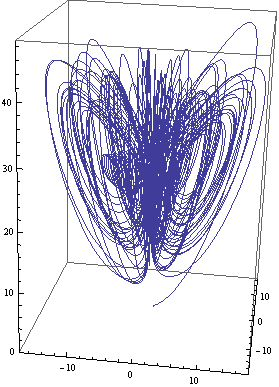
\includegraphics[width=\textwidth,clip=true]
                        {CLEx1x2z} %CLEx1x2zRelEqu}
		\end{exampleblock}
	\end{columns}
\end{frame}

\begin{frame}{} %{\statesp\ portrait of \cLf\ solutions}
\begin{block}{continuous symmetry induces drifts}
\begin{center}
  \includegraphics[width=0.35\textwidth,clip=true] %,height=0.5\textheight
  {CLEchaotic}
  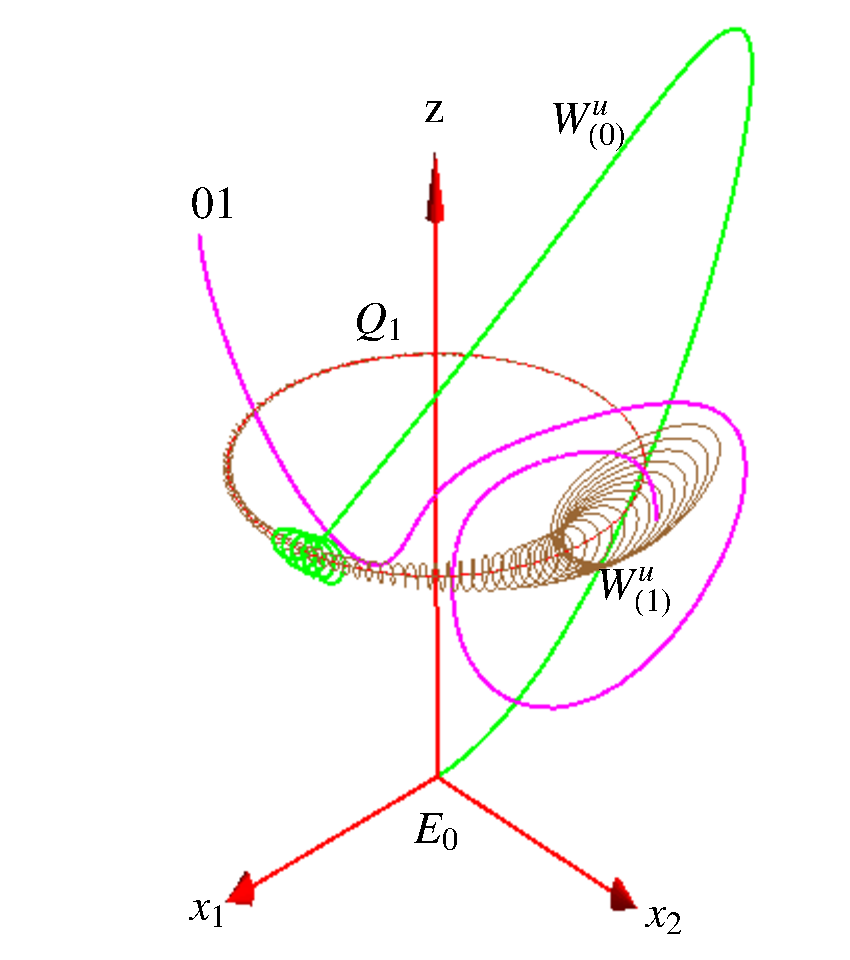
\includegraphics[width=0.35\textwidth,clip=true]
  {CLEcompact}
\end{center}
\end{block}
\begin{itemize}
  \item generic chaotic trajectory (blue)
  \item $E_0$ \eqv  %\EQV{0}
  \item $E_0$ unstable manifold - a cone of such (green)
  \item $Q_1$ \reqv\ (red)
  \item $Q_1$ unstable manifold, one for each point on $Q_1$ (brown)
  \item \rpo\ \cycle{01} (purple)
\end{itemize}
\end{frame}

\begin{frame}{\Large die L\"osung}
% \begin{frame}{from {\cLf} $5D$ attractor $\to$ unimodal map}
	\begin{columns}[t]
	\column{.6\textwidth}
		\only<1>{
			\begin{block}{what to do?}
it's a mess
			\end{block}
			\begin{block}{the goal}
 reduce this messy strange attractor
to something simple
			\end{block}
			}
		\only<2-3>{
			\begin{block}{the goal attained}
			\end{block}
			\begin{block}{but it will cost you}
must learn how to
reduce (quotient) the $\SOn{2}$ symmetry
			\end{block}
			}
	\column{.40\textwidth}
    	\only<1>{
		\begin{exampleblock}{attractor}
        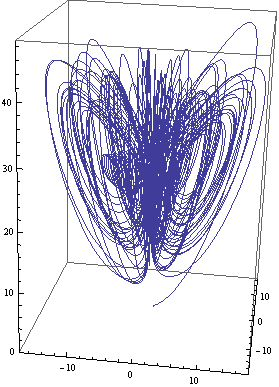
\includegraphics[width=\textwidth,clip=true]
                        {CLEx1x2z} %CLEx1x2zRelEqu}
		\end{exampleblock}
        }
        \only<2-3>{
		\begin{exampleblock}{1D return map!}
        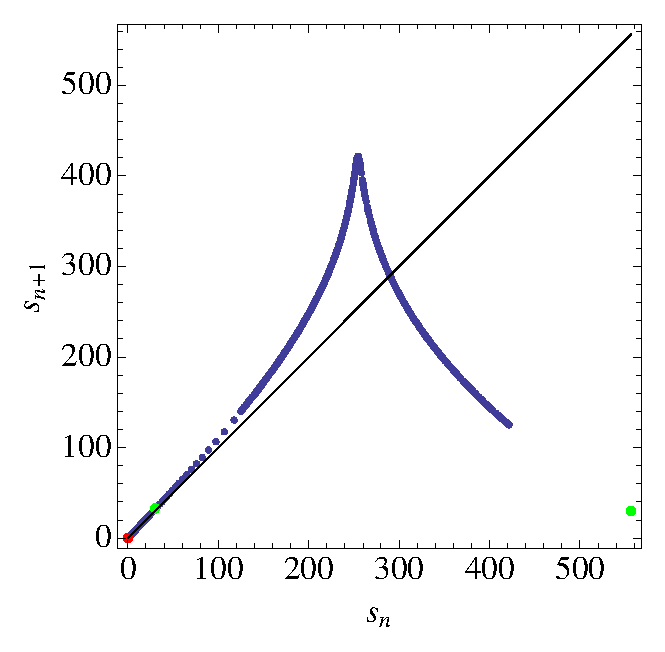
\includegraphics[width=\textwidth,clip=true]
                        {CLEipRM}
		\end{exampleblock}
        }
	\end{columns}
        \only<3>{

\bigskip
\textcolor{red}{\Large how?} hang on, that's what we'll explain here
        }
\end{frame}

\section[relativity for cyclists]{relativity for cyclists}

\subsection[in/equivariance]{}

\begin{frame}{symmetries of dynamics}
\begin{block}{a flow $\dot{\ssp}= \vel(\ssp)$ is $\Group$-equivariant if}
\[
\vel(\ssp)=\LieEl^{-1} \, \vel(\LieEl \, \ssp)
\,,\qquad \mbox{for all } \LieEl \in {\Group}
\,.
\] %ee{eq:FiniteRot}
\end{block}

\bigskip
\begin{block}{definition: Lie group}
a topological group $\Group$ such that
\\
     (1) $\Group$ has the structure of a smooth differential manifold
\\
     (2) composition map
     $\Group \times \Group \to \Group: (g,h) \to g h^{-1}$ is smooth
\end{block}


\bigskip
mystified?

\bigskip
just think
``aha, like the rotation group \SOn{3}...''
\end{frame}

\begin{frame}{example: \SOn{2} invariance}
			\begin{exampleblock}{{\cLe}}
\scriptsize		
\[
		\left[
					\begin{array}{c}
				\dot{x}_1 \\ \dot{x}_2 \\ \dot{y}_1 \\ \dot{y}_2 \\ \dot{z}
				\end{array}
		\right]
=
		\left[
					\begin{array}{c}
				 -\sigma x_1 + \sigma y_1 \\
				-\sigma x_2 + \sigma y_2 \\
                (\RerCLor-z) x_1 - \ImrCLor x_2 -y_1-e y_2 \\
                \ImrCLor x_1 + (\RerCLor-z) x_2 + e y_1- y_2 \\
				-b z + x_1 y_1 + x_2 y_2
				\end{array}
		\right]
\]
			\end{exampleblock}

\begin{block}{}
invariant under a \SOn{2} rotation by finite angle
\gSpace:
\scriptsize		
\[
\LieEl(\gSpace) \,=\,  \left(\barr{ccccc}
  \cos \gSpace  & \sin \gSpace  & 0 & 0 & 0 \\
 -\sin \gSpace  & \cos \gSpace  & 0 & 0 & 0 \\
 0 & 0 &  \cos \gSpace & \sin \gSpace   & 0 \\
 0 & 0 & -\sin \gSpace & \cos \gSpace   & 0 \\
 0 & 0 & 0             & 0              & 1
    \earr\right)
\] %{CLfRots}
\end{block}
%\begin{block}{\statesp\ decomposition}
%\begin{enumerate}
%  \item $m=0$ \SOn{2}-invariant subspace: $z$-axis
%  \item $m=1$ subspace with multiplicity 2
%\end{enumerate}
%\end{block}
\end{frame}

\begin{frame}{example: abelian group $\SOn{2}$}
% { \label{exmp:SO2rot}

$\SOn{2}$ : rotations in a plane

\hfill \textcolor{red}{\scriptsize
reflection $(x,y) \to (-x,y)$ excluded ($\det \LieEl = -1$)
}

\bigskip\bigskip
if the group $\Group$ actions consists of two such rotations which
commute,
% for example a $3D$ box or pipe with two periodic boundary conditions,
the group $\Group$ is an Abelian group that sweeps out a
$T^2$ torus
\end{frame}

\begin{frame}{example: continuous symmetries of pipe flow}
%{    \label{exmp:PpCfSymm}
	\begin{columns}[t]
	\column{.6\textwidth}
			\begin{exampleblock}{pipe flow}
\begin{itemize}
  \item     periodic streamwise, spanwise
  \item     eqs. under azimuthal flip invariant
  \item[a)] $\SOn{2}_z\times \On{2}_\theta$ symmetry
  \item[b)] laminar sol. is invariant
\end{itemize}
			\end{exampleblock}
	\column{.40\textwidth}
            \begin{block}{}
        \includegraphics[width=\textwidth,clip=true]
                        {500px-Poiseuille_abstraction}
			\end{block}
	\end{columns}
\end{frame}

\begin{frame}{group orbits}
for any $\ssp \in \pS$, the
\textcolor{blue}{group orbit} $\pS_\ssp $ of $\ssp$ is the set of all group
actions
\[
\pS_\ssp = \{g\,\ssp \mid g \in {\Group}\} \subset \pS
\]

\bigskip\bigskip
states in $\pS_\ssp $ are physically equivalent
\end{frame}

\begin{frame}{example: group orbit of a pipe flow  \reqv}
{\scriptsize
\slicep\ = Kerswell \emph{et al} $N2\_M1$ solution,
($\Reynolds =2400$, stubby $L=2.5D$ pipe)
}

\medskip

a very smooth, almost laminar solution

	\begin{columns}[t]
	\column{.45\textwidth}
			\begin{exampleblock}
{$\SOn{2}\times\SOn{2}$ symmetry
\\
$\Rightarrow$
group orbit is 2-torus}
projected on
  \begin{itemize}
    \item 2 \slicep\ group tangents
    \item 3. axis along the curvature direction
  \end{itemize}
			\end{exampleblock}
	\column{0.55\textwidth}
\begin{block}
  \centering
\includegraphics[width=1.00\textwidth]{2839GOLB} %{2830GO7}
%  \caption{\label{fig:2830GO6}
    %\label{fig:M1groupOrb}
\end{block}
	\end{columns}

\bigskip
{\scriptsize
$2d$ group orbit (in 100,000 dimension \textcolor{red}{\statesp}) traced out by
  \begin{itemize}
    \item equal increment translations in $\theta$ (dashed blue)
    \item equal increments in $z$ (solid red)
  \end{itemize}
}
\end{frame}

\begin{frame}{example: group orbit of a pipe flow turbulent state}
{\scriptsize
\slicep\ is Kerswell \emph{et al} $N2\_M1$  \reqv
\\
( $\Reynolds =2400$,
stubby $L=2.5D$ pipe)
}

\medskip

a turbulent state


	\begin{columns}[t]
	\column{.45\textwidth}
			\begin{exampleblock}
{$\SOn{2}\times\SOn{2}$ symmetry
\\
$\Rightarrow$
group orbit is 2-torus}
			\end{exampleblock}
	\column{0.55\textwidth}
\begin{block}
  \centering
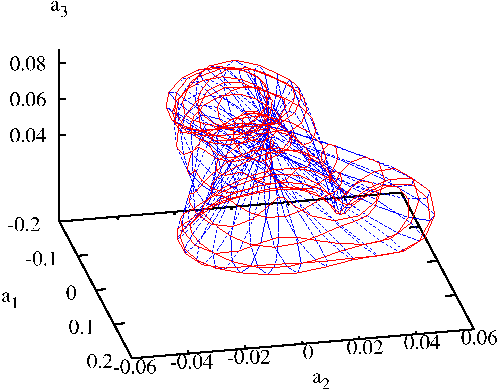
\includegraphics[width=1.00\textwidth]{2840GOt135M1} %{2830GO7}
%  \caption{\label{fig:2830GO6}
    %\label{fig:M1groupOrb}
\end{block}
	\end{columns}

\bigskip
group orbits of nonlinear states are highly contorted
\end{frame}

\begin{frame}{foliation by group orbits}
  \begin{columns}
  \column{0.5\textwidth}
\begin{block}{group orbits}
% 2011-08-23 Predrag: previously BeThTraj.pdf from
% dasbuch/book/FigSrc/inkscape/BeThTraj.svg
%  2011-09-09 Predrag: updated continuous.tex overheads
%  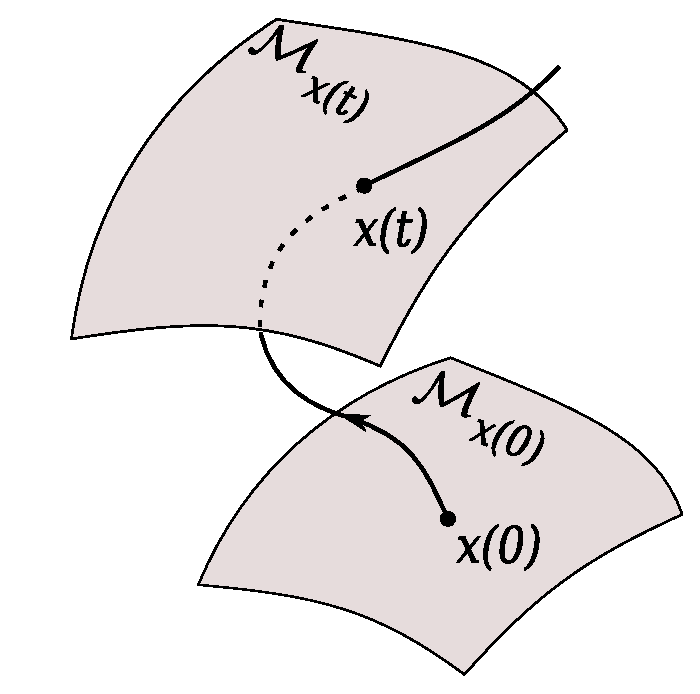
\includegraphics[width=1.00\textwidth,clip=true]{BeThTraj}
 \begin{center}
  \setlength{\unitlength}{1.00\textwidth}
  %% \unitlength = units used in the Picture Environment
  \begin{picture}(1,1.07471658)%
    \put(0,0){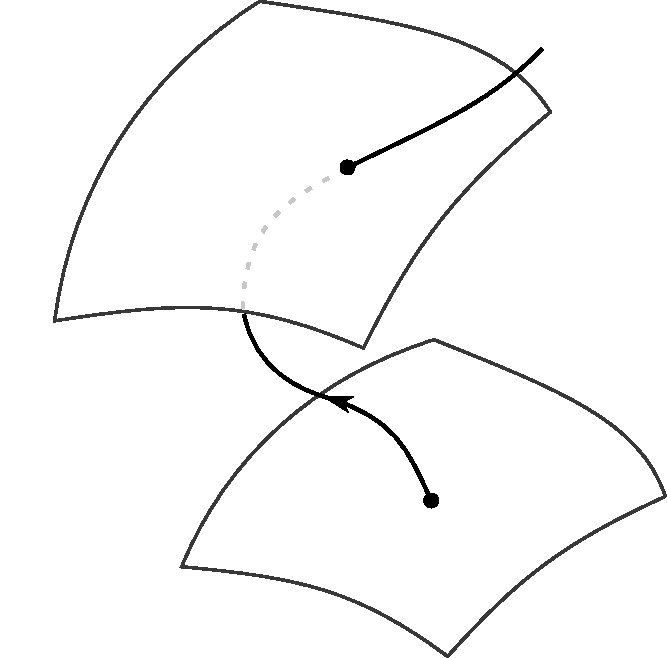
\includegraphics[width=\unitlength]{BeThTrajTeX}}%
    \put(0.28879298,1.02196543){\color[rgb]{0,0,0}\rotatebox{-22.37140782}{\makebox(0,0)[lb]{\smash{$\pS_{\ssp(\tau)}$}}}}%
    \put(0.55566402,0.45078735){\color[rgb]{0,0,0}\rotatebox{-16.6673442}{\makebox(0,0)[lb]{\smash{$\pS_{\ssp(0)}$}}}}%
    \put(0.63028127,0.18433597){\color[rgb]{0,0,0}\rotatebox{0.03136739}{\makebox(0,0)[lb]{\smash{$\ssp(0)$}}}}%
    \put(0.46253394,0.70182304){\color[rgb]{0,0,0}\rotatebox{0.03136739}{\makebox(0,0)[lb]{\smash{$\ssp(\tau)$}}}}%
    \put(0.03852492,0.09250899){\color[rgb]{0,0,0}\rotatebox{0.11031334}{\makebox(0,0)[lb]{\smash{$\pS$}}}}%
  \end{picture}%
 \end{center}
\end{block}
  \column{0.5\textwidth}
		\only<1>{
\noindent
\emph{group orbit} $\pS_\ssp $ of $\ssp$ is the set of all group
actions
\[
\pS_\ssp = \{\LieEl\,\ssp \mid \LieEl \in {\Group}\}
\]
        }
		\only<2>{
%\noindent
%group orbit $\pS_{\ssp(0)}$ of \statesp\ point
% $\ssp(0)$, and the group orbit $\pS_{\ssp(t)}$
%reached by the trajectory $\ssp(t)$ time $t$ later.
%        }
%		\only<3>{
\noindent
any point on the manifold $\pS_{\ssp(t)}$ is
equivalent to any other
        }
		\only<3>{
\noindent
action of a symmetry group
foliates the \statesp\ into a union of group
orbits

\medskip

each group orbit an equivalence class
        }
\end{columns}
\end{frame}

\section{symmetry reduction}

\begin{frame}{}
\begin{block}{the goal}
replace each group orbit by a unique
point in a lower-dimensional

\bigskip

\hfill
\textcolor{red}{\Large symmetry \reducedsp\ $\pS/\Group$}
\end{block}
\end{frame}

\begin{frame}{symmetry reduction}
  \begin{columns}
  \column{0.5\textwidth}
\begin{block}{full \statesp}
 \begin{center}
  \setlength{\unitlength}{1.00\textwidth}
  %% \unitlength = units used in the Picture Environment
  \begin{picture}(1,1.07315413)%
    \put(0,0){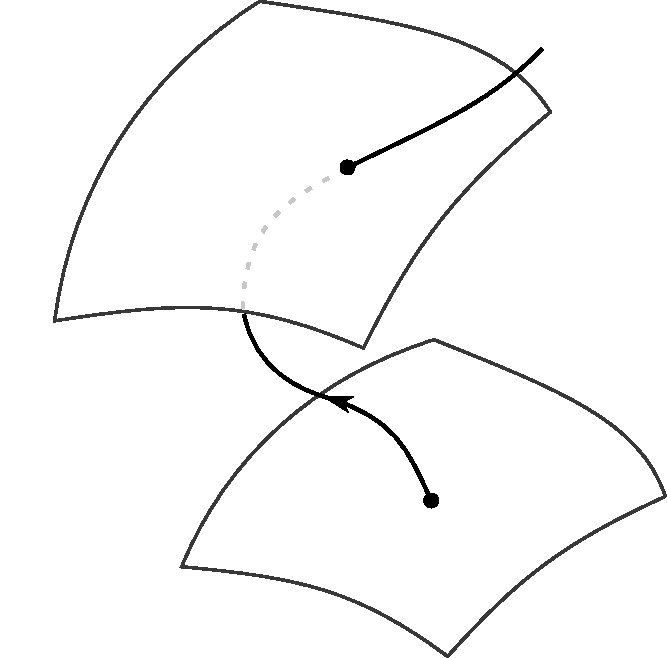
\includegraphics[width=\unitlength]{BeThTrajTeX}}%
    \put(0.30362031,0.99939308){\color[rgb]{0,0,0}\rotatebox{-31.32889204}{\makebox(0,0)[lb]{\smash{$\pS_{\ssp(\tau)}$}}}}%
    \put(0.5686188,0.45975596){\color[rgb]{0,0,0}\rotatebox{-40.8073288}{\makebox(0,0)[lb]{\smash{$\pS_{\ssp(0)}$}}}}%
    \put(0.63028127,0.18433598){\color[rgb]{0,0,0}\rotatebox{0.03136739}{\makebox(0,0)[lb]{\smash{$\ssp(0)$}}}}%
    \put(0.46253394,0.70182305){\color[rgb]{0,0,0}\rotatebox{0.03136739}{\makebox(0,0)[lb]{\smash{$\ssp(\tau)$}}}}%
  \end{picture}%
 \end{center}
\end{block}
  \column{0.5\textwidth}
\begin{block}{\reducedsp}
 \begin{center}
  \setlength{\unitlength}{1.00\textwidth}
  %% \unitlength = units used in the Picture Environment
  \begin{picture}(1,1.07315413)%
    \put(0,0){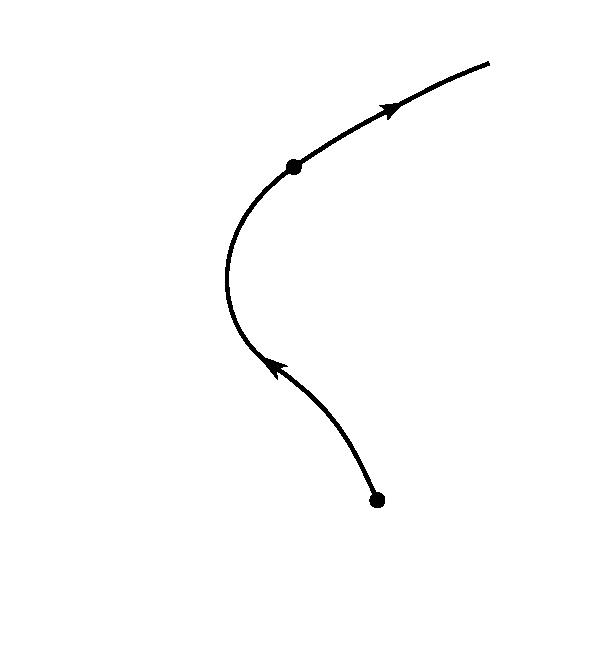
\includegraphics[width=\unitlength]{BeThRedTeX}}%
    \put(0.19912369,0.17144733){\color[rgb]{0,0,0}\rotatebox{0.11031334}{\makebox(0,0)[lb]{\smash{$\pSRed$}}}}%
    \put(0.63028127,0.18433598){\color[rgb]{0,0,0}\rotatebox{0.03136739}{\makebox(0,0)[lb]{\smash{$\sspRed(0)$}}}}%
    \put(0.46253394,0.70182305){\color[rgb]{0,0,0}\rotatebox{0.03136739}{\makebox(0,0)[lb]{\smash{$\sspRed(\tau)$}}}}%
  \end{picture}%
 \end{center}
\end{block}
\end{columns}
\end{frame}


\begin{frame}{pedestrian attempt : \reqv\ or `traveling wave'}
\includegraphics[width=0.8\textwidth,clip=true]{AW-TW2}

dynamical orbit confined to the group orbit
\[
\LieEl(\tau) \, \ssp(0) =
\ssp(\tau) \in \pS_{\REQV{}{}}
\]
\end{frame}

\begin{frame}{pedestrian${}^*$ attempt : moving frame}
\includegraphics[width=0.8\textwidth,clip=true]{AW-TW3}

\reqv\ is made stationary by
\\
a counter-rotating `frame'

\vfill
\textcolor{yellow}
{\scriptsize ${}^*$ `pedestrian' = polite word for `applied mathematician'}
\end{frame}

\subsection{\rpo s}
%\label{s-rpos}

\begin{frame}{\rpo}
A \rpo\ $p$ is an orbit in
{\statesp} $\pS$ which exactly recurs
%    \PC{create SFIG here}
\beq
\ssp_p (t) = g_p \ssp_p (t + \period{p} )
    \,,\qquad
\ssp_p (t) \in \pS_p
\label{RPOrelper1}
\eeq
for a fixed \textcolor{blue}{relative period} $\period{p}$
and a fixed group action ${g_p} \in  \Group$
that ``rotates" the endpoint $\ssp_p (\period{p} ) $
back into the initial point $\ssp_p (0) $.
\end{frame}

\begin{frame}{\rpo\ : \statesp\ visualization}
  \begin{columns}
  \column{0.55\textwidth}
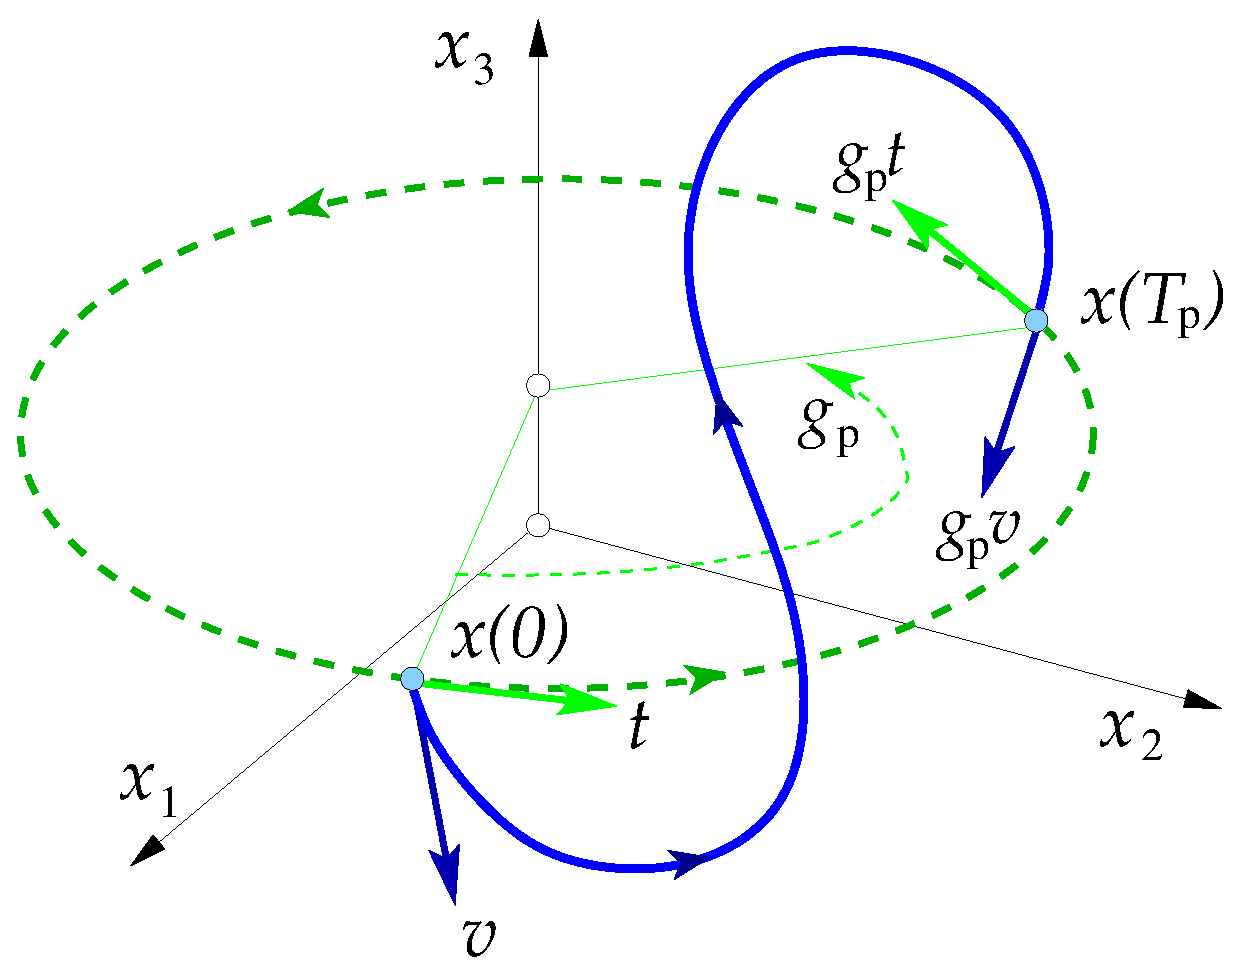
\includegraphics[width=1.0\textwidth,clip=true]
    {rpo}
  \column{0.45\textwidth}
		\only<1>{
\noindent
each cycle point
\begin{block}{}
\hfill
$\ssp_p (0) = \LieEl_p \ssp_p (\period{p} )
$ %\label{RPOrelper1}
\end{block}
exactly recurs at a fixed
\begin{block}{relative period} \hfill $\period{p}$
\end{block}
but shifted by a fixed
\begin{block}{group action} \hfill ${\LieEl_p}$
\end{block}
        }
		\only<2>{
\noindent
group action parameters
\\
$\gSpace = (\gSpace_1,\gSpace_2,\cdots\gSpace_N)$
are\\
irrational:

\bigskip

trajectory sweeps out ergodically the group orbit without
ever closing into a \po
        }
\end{columns}
		\only<1>{
{\scriptsize \textcolor{green}
{(green dashes) group orbit}\\
\textcolor{blue}{(blue) \rpo\ orbit}\\
(arrows) \textcolor{blue}{velocity}, \textcolor{green}{group} tangents
}
            }
\end{frame}

\begin{frame}{example : pipe flow \rpo\ $\RPO{36.72}$}
symmetry reduction: full \statesp\ trajectory $\ssp(t)$

\begin{center}$\Rightarrow$\end{center}

\reducedsp\ trajectory $\sspRed(t)$, continuous
group induced drifts quotiented out
  \begin{columns}
  \column{0.5\textwidth}
\begin{block}{full \statesp}
 \begin{center}
  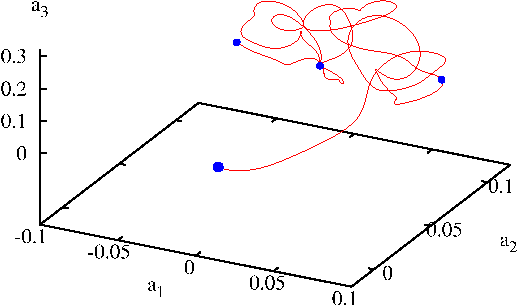
\includegraphics[width=\textwidth]{2841GO3a}
 \end{center}
{\scriptsize traced for two periods:}
\\
{\scriptsize fills quasi-periodically
a highly contorted 2-torus }
\end{block}
  \column{0.5\textwidth}
\begin{block}{\reducedsp}
 \begin{center}
  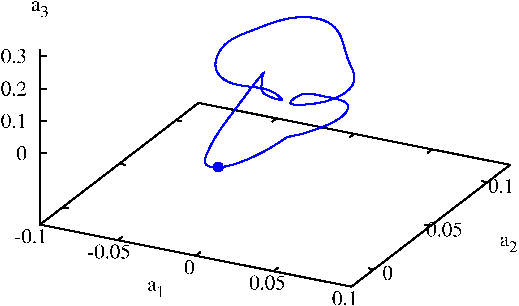
\includegraphics[width=\textwidth]{2841GO3b}
 \end{center}
{\scriptsize
closes a \po\ in one period}
\end{block}
\end{columns}
\end{frame}

\begin{frame}{relativity for pedestrians}
		\only<1,2>{
\begin{block}{try a co-moving coordinate frame?}
        }
		\only<3>{
\begin{block}{no good global co-moving frame!}
        }
\begin{center}
		\only<1>{
(\textit{a})
  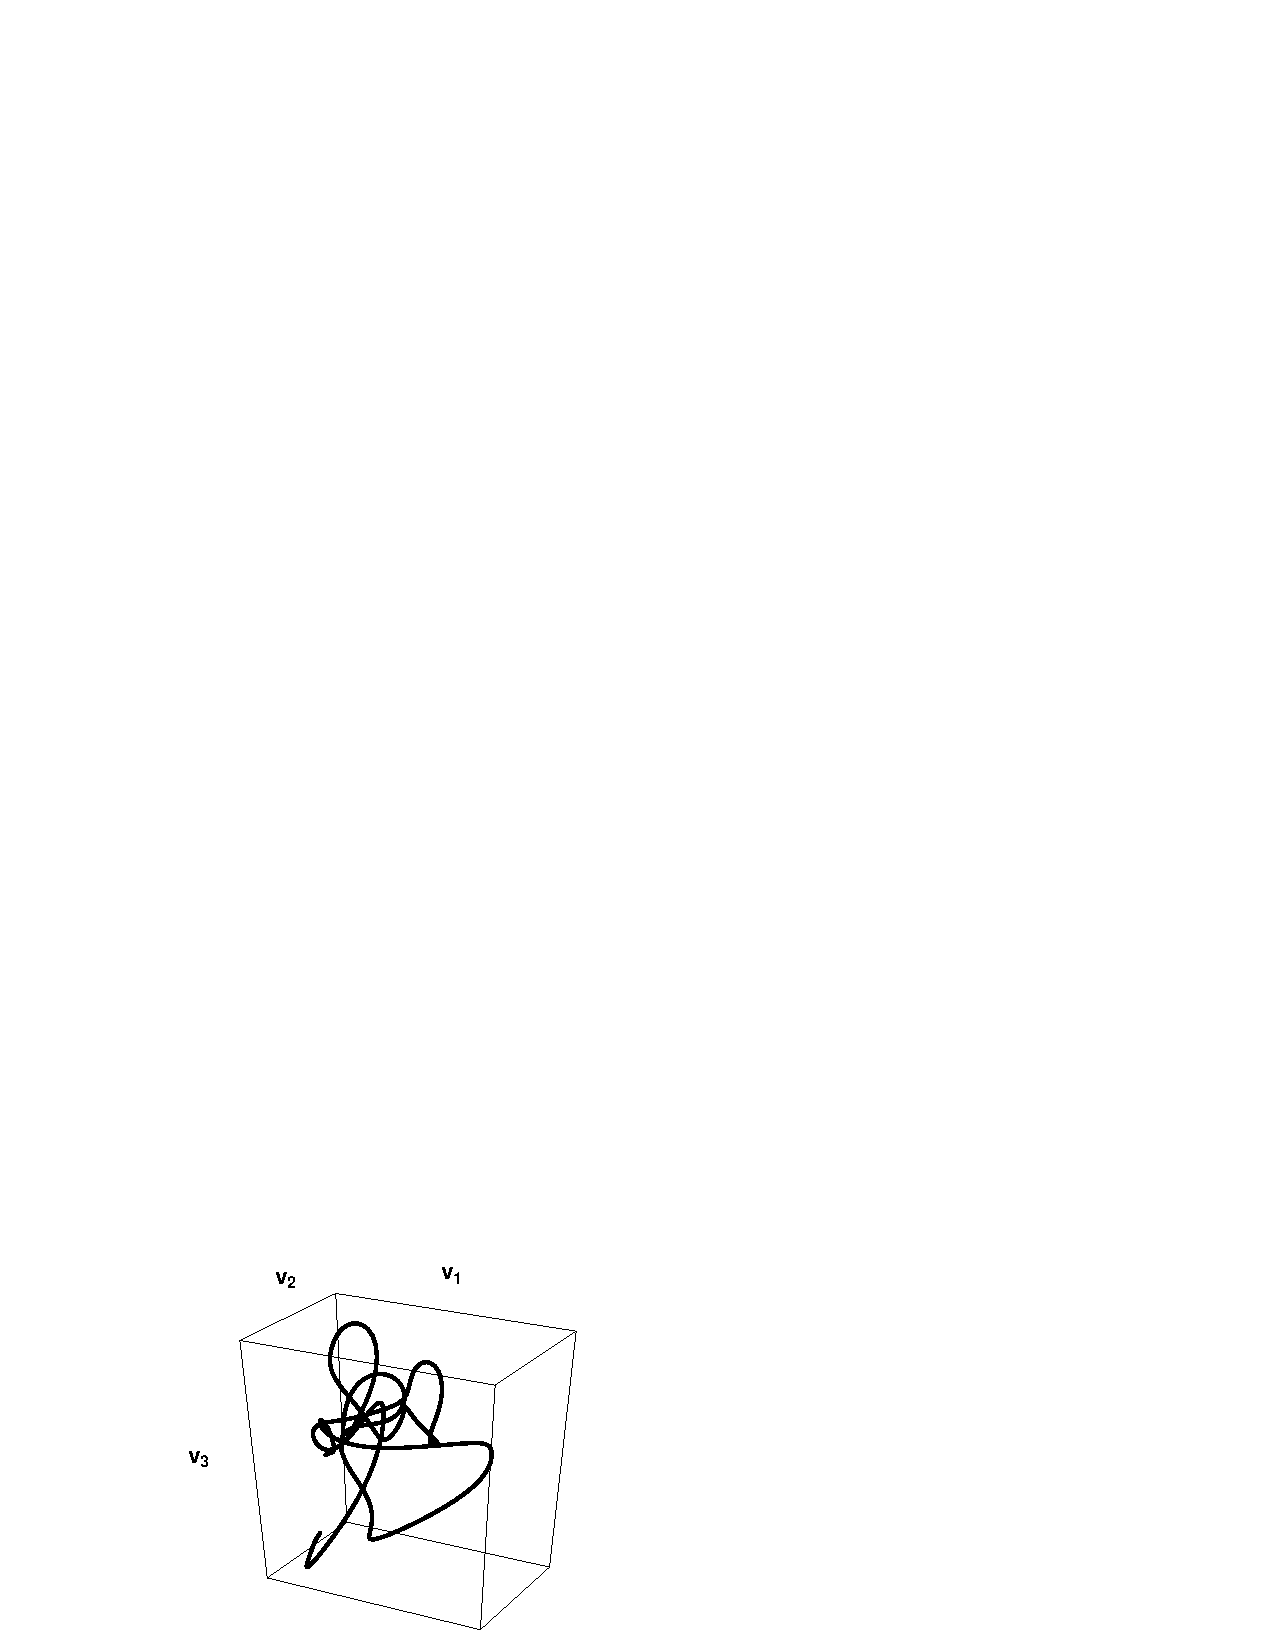
\includegraphics[width=0.40\textwidth,height=0.5\textheight,clip=true]
  {ks22rpo033p50_04p045E2}
        }
		\only<2,3>{
(\textit{b})
  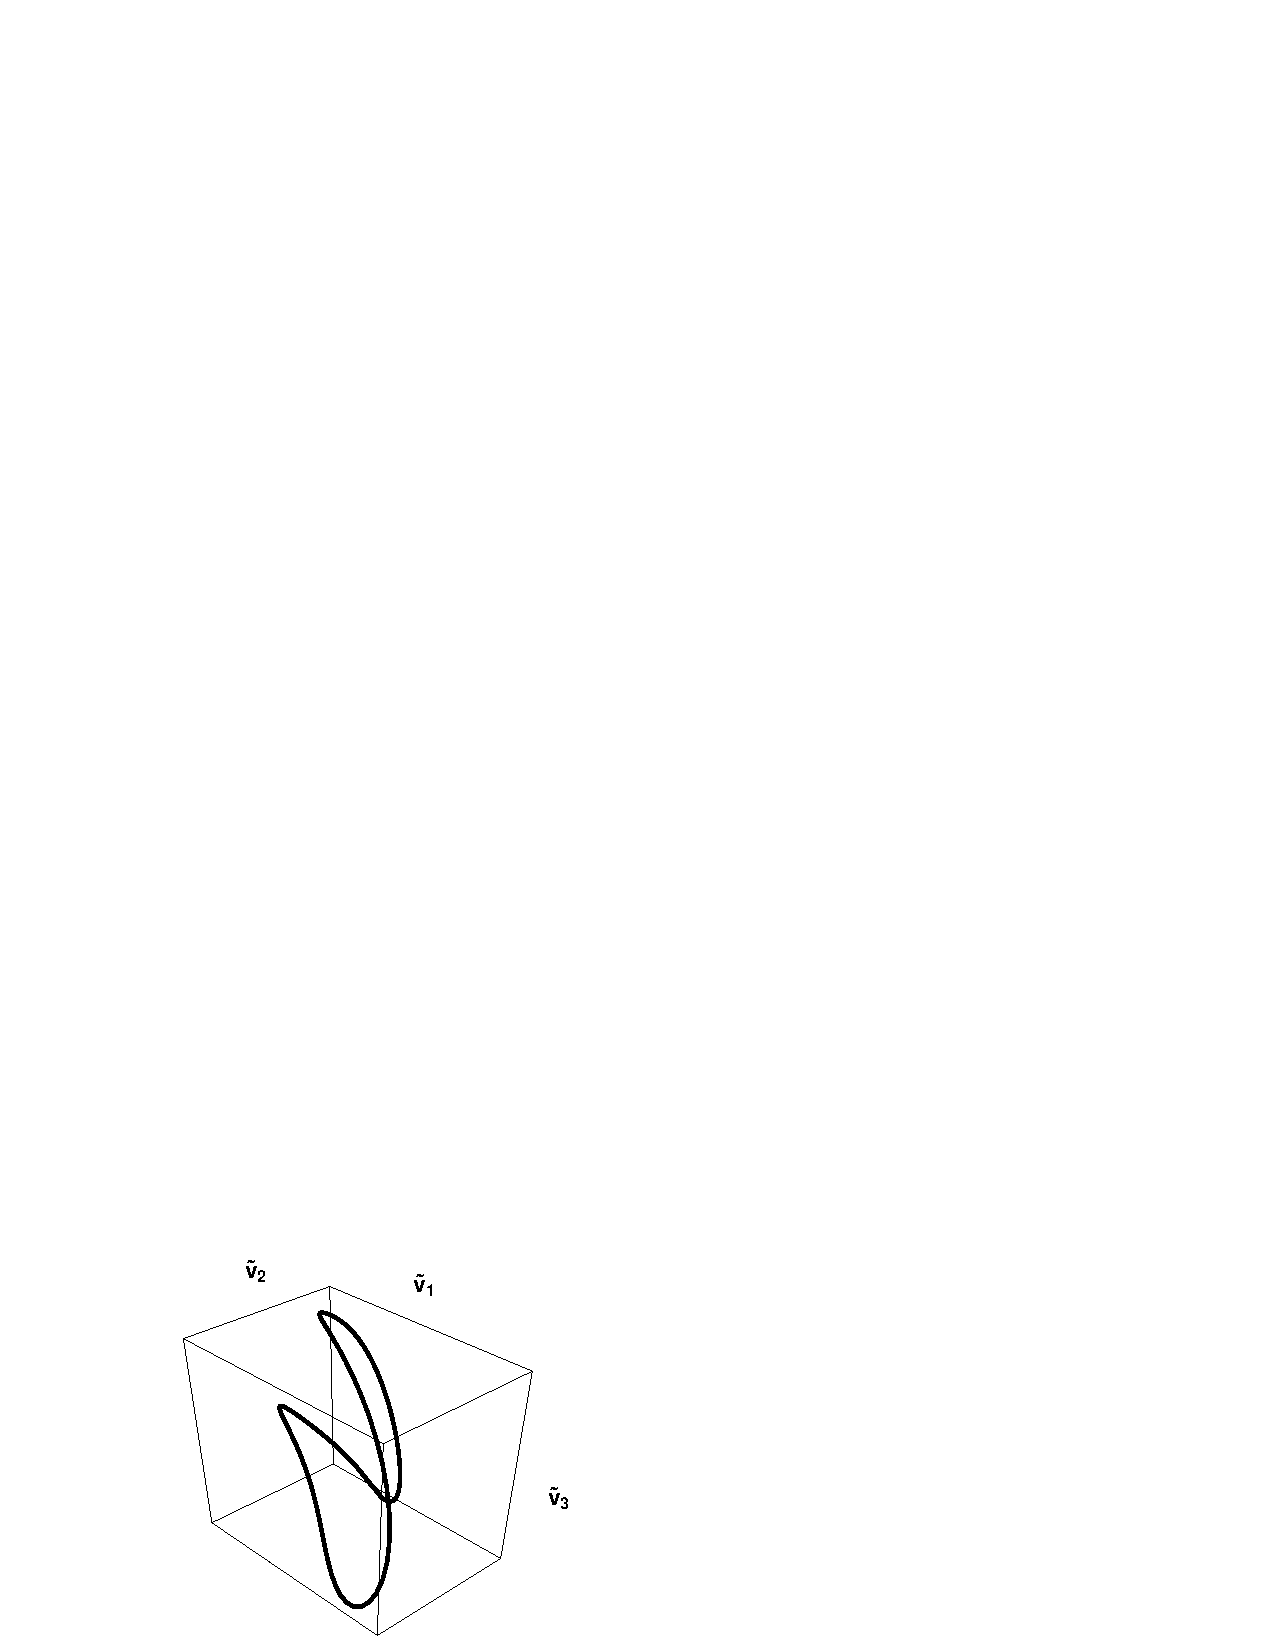
\includegraphics[width=0.40\textwidth,height=0.5\textheight,clip=true]
  {ks22rpo033p50_04p045E2CM}
        }
\end{center}
\end{block}
		\only<1>{
a \rpo\ of the Kuramoto-Sivashinsky flow, 128$d$ \statesp\
traced for four periods
 $\period{p}$, projected on

\bigskip
a stationary \statesp\ coordinate frame
 $\{v_1,v_2,v_3\}$; a mess
        }
		\only<2>{
a \rpo\ of the Kuramoto-Sivashinsky flow projected on

\bigskip
a co-moving $\{\tilde{v}_1,\tilde{v}_2,\tilde{v}_3\}$ frame
        }
        \only<3>{
beautiful, but
this is no symmetry reduction at all;

\bigskip
all other \rpo s require their own frames,
 \\
 moving at different velocities!
        }
\end{frame}


\section[slice n' dice]{slice n' dice}


\begin{frame}{relativity for cyclists}
\begin{block}{method of moving frames / slices}

\bigskip
cut group orbits by a hypersurface (kind of
Poincar\'e section), each group orbit of
symmetry-equivalent points represented by the single point
\end{block}
\bigskip
\textcolor{red}{\Large cut how?}
\end{frame}


\begin{frame}{inspiration: pattern recognition}
you are observing turbulence in a pipe flow, or your defibrillator has a
mesh of sensors measuring electrical currents that cross your heart, and

\medskip

you have a precomputed pattern, and are sifting through the data set of
observed patterns for something like it

\medskip

here you see a pattern, and there you see a pattern that seems much like
the first one

\bigskip

\bigskip

\textcolor{red}{\Large how `much like the first one?'}
\end{frame}

\begin{frame}{}
take the first pattern
\begin{block}{`template' or `reference state'}
\hfill  a point {\slicep} in the \statesp\  \pS
\end{block}

and use the symmetries of the flow to
\begin{block}{slide and rotate the `{\template}'}
\hfill  act with elements of the symmetry group \Group\ on
$\slicep \to \LieEl(\gSpace)\,\slicep$
\end{block}
 until it overlies the second pattern (a point $\ssp$ in
the \statesp)
\begin{block}{distance between the two patterns}
\[ %beq
|\ssp - \LieEl(\gSpace)\,\slicep|
    = |\sspRed - \slicep|
%\label{minDistance}
\] %eeq
\end{block}
is minimized
\end{frame}

\begin{frame}{idea: the closest match}
  \begin{columns}
  \column{0.60\textwidth}
\begin{block}{} %group orbits}
\begin{center}
  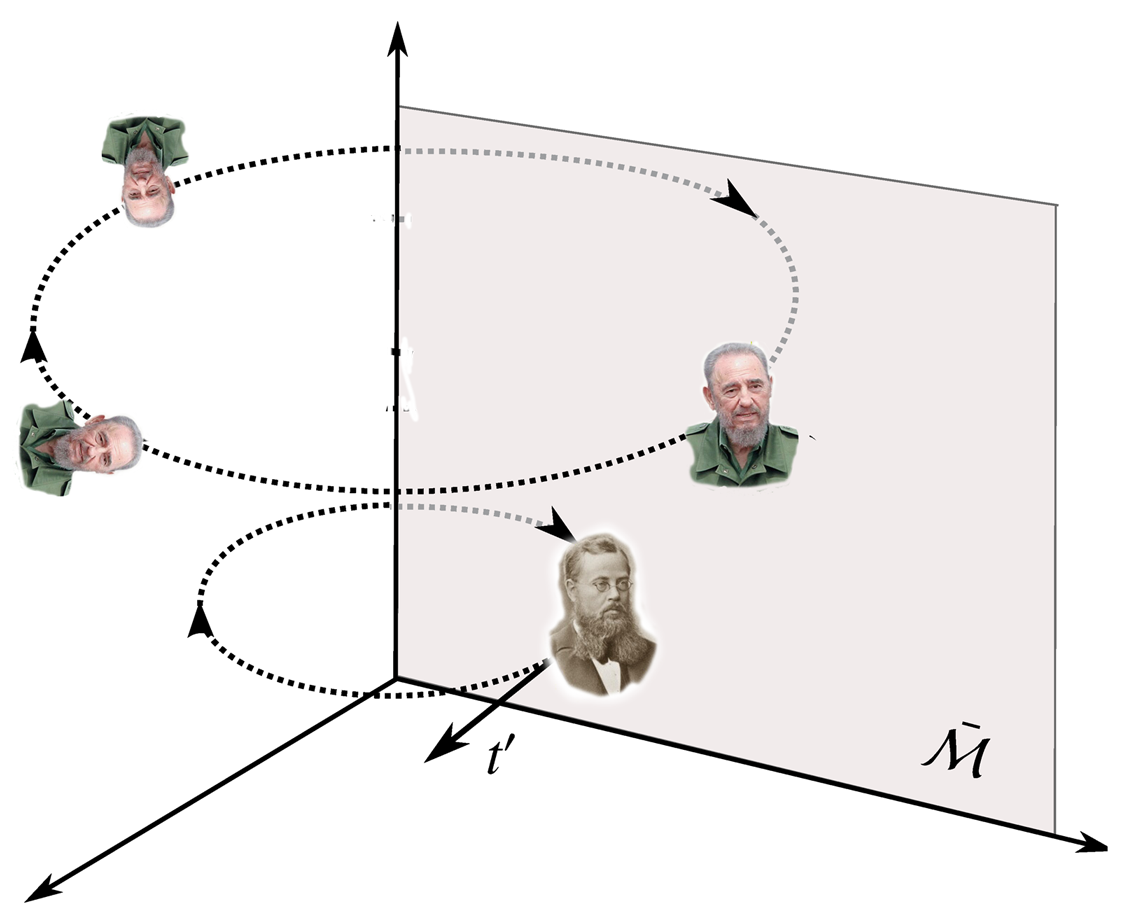
\includegraphics[width=1.00\textwidth,clip=true]
  {sliceLie}
\end{center}
\end{block}
  \column{0.40\textwidth}
template: Sophus Lie

\bigskip
(1) rotate bearded guy $\ssp$
\\
\textcolor{blue}{traces out the group orbit $\pS_\ssp$}

\bigskip
(2) replace the group orbit by the closest match $\sspRed$
to the template pattern $\slicep$

\bigskip
the closest matches $\sspRed$ lie in the $(d\!-\!N)$ symmetry \reducedsp\
$\pSRed$
\end{columns}
\end{frame}

\begin{frame}{distance}
assume that \Group\
is a subgroup of the group of orthogonal transformations
$\On{d}$, and measure
distance $|\ssp|^2=\braket{\ssp}{\ssp}$ in terms of the Euclidean inner
product

\bigskip
numerical fluids:  PDE discretization independent L2 distance is
\begin{block}{energy norm}
\[
  \Norm{\bu-\bv}^2  = \braket{\bu-\bv}{\bu-\bv}  = \frac{1}{V}
                \int_\bCell \! d \bx \;
                       (\bu-\bv) \cdot (\bu-\bv)
%\label{innerproduct}
\]
\end{block}

\bigskip
experimental fluid:
\begin{block}{image discretization independent distance}
 is Hamming distance, or ???
\end{block}
\end{frame}

\subsection{\mslices}

\begin{frame}{}
\begin{block}{minimal distance}
is a solution to the extremum conditions
\[ %beq
\frac{\partial ~~}{\partial \gSpace_a} |\ssp - \LieEl(\gSpace)\,\slicep|^2
\] % ee{PCsectQ0}
\end{block}
\bigskip
but what is
\[
\frac{\partial ~~}{\partial \gSpace_a} \LieEl(\gSpace)
\,?
\]
\end{frame}

\section{slice \& dice}

\subsection[Lie groups]{Lie groups for pedestrians}
% \subsection{Group representations}
% \subsection{Compact groups}
% Predrag                               13 aug 2006
% extracted from GroupTheory webbook
% \Chapter{grint}{August 13, 2006}{Group integrals}

\begin{frame}{Lie algebras for pedestrians}
an element of a compact Lie group:
\[
\LieEl(\gSpace) \propto e^{\gSpace \cdot \Lg }
	\,,\qquad
\gSpace \cdot \Lg  = \sum \gSpace_a \Lg_a,\; a=1,2, \cdots, N
\] %ee{FiniteRot}
$\gSpace \cdot \Lg$: {\em Lie algebra} element
\\
$\gSpace_a$: parameters of the transformation.

\bigskip
\begin{block}{infinitesimal transformations}
\[
g=e^{\delta \gSpace \cdot \Lg}
 \simeq  1 + \gSpace \cdot \Lg \,, \qquad \vert \delta \gSpace \vert \ll 1
\]
\end{block}
\begin{block}{Lie algebra}
\begin{itemize}
  \item $T_a$ are \textcolor{blue}{generators} of infinitesimal
transformations
  \item here $T_a$ are $[d\!\times\!d]$ antisymmetric matrices
  \item $T_a$ are elements of the Lie algebra of $\Group$
\end{itemize}
\end{block}
\end{frame}

\begin{frame}{example: \SOn{2} invariance of \cLe}
\cLe\ equations are invariant under
\\
\SOn{2} rotation by finite angle \gSpace:
\[
\LieEl(\gSpace) \,=\,  \left(\barr{ccccc}
  \cos \gSpace  & \sin \gSpace  & 0 & 0 & 0 \\
 -\sin \gSpace  & \cos \gSpace  & 0 & 0 & 0 \\
 0 & 0 &  \cos \gSpace & \sin \gSpace   & 0 \\
 0 & 0 & -\sin \gSpace & \cos \gSpace   & 0 \\
 0 & 0 & 0             & 0              & 1
    \earr\right)
\] %{CLfRots}
%\begin{frame}{example:
\SOn{2} Lie algebra has one generator
of infinitesimal rotations
\[
 \Lg \,=\,   \left(\barr{ccccc}
    0  &  1 & 0  &  0 & 0  \\
   -1  &  0 & 0  &  0 & 0 \\
    0  &  0 & 0  &  1 & 0  \\
    0  &  0 &-1  &  0 & 0 \\
    0  &  0 & 0  &  0 & 0
    \earr\right)
\] %ee{CLfLieGen}
\end{frame}

\begin{frame}{now have the `slice condition'}
\begin{block}{group tangent fields}
flow field at the \statesp\
point $\ssp$ induced by the action of the group is given by
the set of $N$ \emph{tangent fields}
\[
\groupTan_a(\ssp)_{i}= (\Lg_a){}_{ij} \ssp_j
\] %{GroupTangField}
\end{block}
\bigskip
\begin{block}{slice condition}
\[ %beq
\frac{\partial ~~}{\partial \gSpace_a} |\ssp - \LieEl(\gSpace)\,\slicep|^2
   =
2\, \braket{\sspRed - \slicep}{\sliceTan{a}}
   = 0
    \,,\qquad
	  \sliceTan{a} = \Lg_a \slicep
\] % ee{PCsectQ0}
\end{block}
\end{frame}

\begin{frame}{traveling wave}
\includegraphics[width=0.8\textwidth,clip=true]{AW-TW5}
\end{frame}

%\begin{frame}{traveling wave}
%\includegraphics[width=0.8\textwidth,clip=true]{AW-TW6}
%\end{frame}

\begin{frame}{traveling wave}
\includegraphics[width=0.8\textwidth,clip=true]{AW-TW4}
\end{frame}

\begin{frame}{flow within the slice}
\slice\ fixed by \slicep

\bigskip
	\begin{exampleblock}
          {\reducedsp\ $\pSRed$  flow $\velRed(\sspRed)$}
\bea
\velRed(\sspRed) &=& \vel(\sspRed)
                    \,-\, \dot{\gSpace}(\sspRed)  \cdot \groupTan(\sspRed)
    \,,\qquad\quad \sspRed \in \pSRed
\continue
\dot{\gSpace}_a(\sspRed) &=& (\vel(\sspRed)^T \sliceTan{a})
                       /(\groupTan(\sspRed)^T \cdot \sliceTan{})
\,.
\nnu %\label{EqMotMFrame}
\eea
	\end{exampleblock}
\begin{itemize}
  \item $\vel$ : velocity, full space
  \item $\velRed$ : velocity component in slice
  \item $\dot{\gSpace}  \cdot \groupTan$ : velocity component normal to slice
  \item $\dot{\gSpace}$ : reconstruction equation for the group phases
\end{itemize}
\begin{block}{Cartan derivative}
\[
\LieEl^{-1}\dot{\LieEl} \,\ssp
    =e^{-\gSpace \cdot \Lg} \,
\frac{d ~~}{d \, \tau} e^{\gSpace \cdot \Lg}\ssp
    =\dot{\gSpace}\cdot \groupTan(\ssp)
\]
\end{block}
\end{frame}

\begin{frame}{flow within the slice}
\begin{block}{} %group orbits}
\begin{center}
  \includegraphics[width=0.70\textwidth,clip=true]
  {sliceRaw}
\end{center}
\end{block}
full-space trajectory $\ssp(\tau)$ \\
rotated into the \reducedsp\ $\sspRed(\tau) = \LieEl(\gSpace)^{-1}\ssp(\tau)$ \\
by appropriate \emph{moving frame} angles $\{\gSpace(\tau)\}$
\end{frame}

%Predrag                                     2011-09-09
%recheck if still used elsewhere, then remove Willis figures
%    talks/figs/ AW-RPO1.pdf AW-RPO2.pdf
%\begin{frame}{\rpo}
%\includegraphics[width=1.0\textwidth,clip=true]{AW-RPO1}
%\end{frame}
%
%\begin{frame}{\rpo}
%\includegraphics[width=1.0\textwidth,clip=true]{AW-RPO2}
%\end{frame}

\begin{frame}{\rpo $\to$ \po}
%%%%%%%%%%%%%%%%%%%%%%%%%%%%%%%%%%%%%%%%%%%%%%%%%%%%%%%%%%%%%%%%
%% slice.*, inflectHype.*: see dasbuch/book/FigSrc/inkscape/00ReadMe.txt
%% rpo.* hand-drawn in dasbuch/book/FigSrc/xfig/rpo.fig
%% xfig exported -> FigSrc/inkscape/rpo.fig
%% inkscape exported -> rpo.eps + LaTeX, hand edited in the macros
%% Predrag 2011-08-27 replaced rpo.pdf by rpoSlice.pdf
%%  2011-09-09 Predrag: updated continuous.tex overheads
%% remember to insert rpoSlice.pdf into ChaosBook
\begin{block}{}
 \begin{center}
  \setlength{\unitlength}{0.70\textwidth}
  %% \unitlength = units used in the Picture Environment
  \begin{picture}(1,0.87085079)%
    \put(0,0){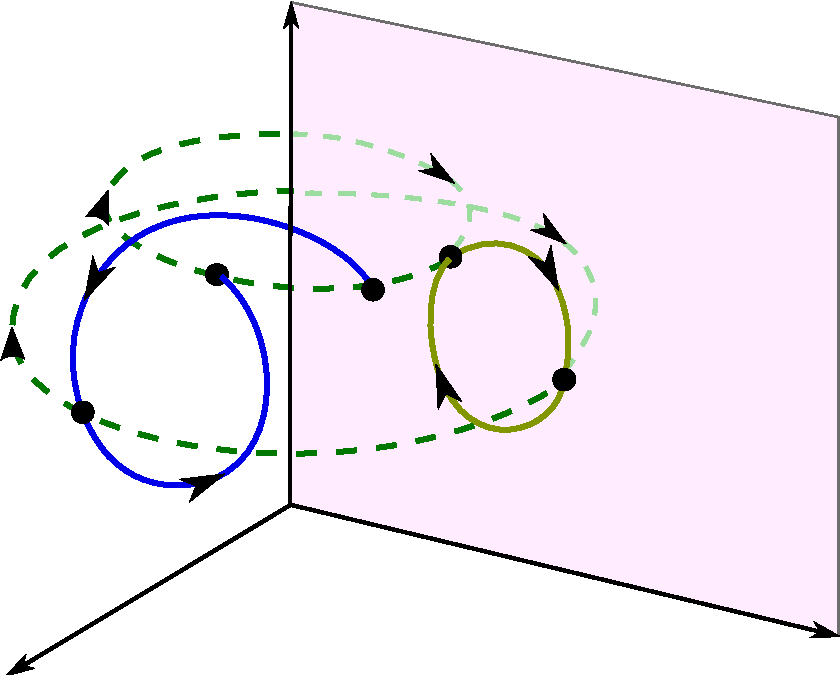
\includegraphics[width=\unitlength]{rpoSlice}}%
    \put(0.82835153,0.19007656){\color[rgb]{0,0,0}\rotatebox{-14.84025432}{\makebox(0,0)[lb]{$\pSRed$}}}%
    \put(0.40925459,0.45713857){\color[rgb]{0,0,0}\rotatebox{0.0313674}{\makebox(0,0)[lb]{\smash{$\ssp(0)$}}}}%
    \put(0.71354118,0.39765314){\color[rgb]{0,0,0}\rotatebox{0.0313674}{\makebox(0,0)[lb]{\smash{$\sspRed(\tau)$}}}}%
    \put(0.13171187,0.38813817){\color[rgb]{0,0,0}\rotatebox{0.0313674}{\makebox(0,0)[lb]{\smash{$\LieEl(\tau)$}}}}%
    \put(0.02168739,0.31359574){\color[rgb]{0,0,0}\rotatebox{0.0313674}{\makebox(0,0)[lb]{\smash{$\ssp(\tau)$}}}}%
    \put(0.15576193,0.48769256){\color[rgb]{0,0,0}\rotatebox{0.0313674}{\makebox(0,0)[lb]{\smash{$\ssp(\period{})$}}}}%
    \put(0.54113911,0.50476963){\color[rgb]{0,0,0}\rotatebox{0.0313674}{\makebox(0,0)[lb]{\smash{$\sspRed(0)$}}}}%
  \end{picture}%
 \end{center}
\end{block}
full \statesp\ \rpo\ $\ssp(\tau)$ \\
is rotated into the \reducedsp\ {\po}
\end{frame}

\begin{frame}{\reqva\ and \rpo s together}
\includegraphics[width=1.0\textwidth,clip=true]{AW-RPO3}
\end{frame}

\begin{frame}{symmetry reduction achieved!}
\begin{itemize}
 \item all points equivalent by symmetries are represented by
    \begin{itemize}
 \item a single point
    \end{itemize}
 \item families of solutions are mapped to a single solution
    \begin{itemize}
 \item \reqva\ become \eqva
 \item \rpo s become \po s
    \end{itemize}
\end{itemize}
\end{frame}

\begin{frame}{take-home message}
rotation into a slice \textcolor{red}{is not} an average\\
 over 3D pipe azimuthal angle

\bigskip\bigskip
it is the full snapshot of the flow embedded in the

\begin{center}
\textcolor{red}{\Large $\infty$-dimensional \statesp}
\end{center}

\bigskip\bigskip
\textcolor{red}{\Large NO information} is lost by symmetry reduction
\begin{itemize}
  \item not modeling by a few degrees of freedom
  \item no dimensional reduction
\end{itemize}
\end{frame}


\begin{frame}{\Large die L\"osung : \cLf\ reduced}
	\begin{columns}[t]
	\column{.50\textwidth}
 		\begin{exampleblock}{full \statesp}
        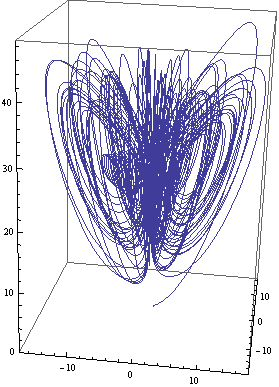
\includegraphics[width=0.7\textwidth,clip=true]
                        {CLEx1x2z} %CLEx1x2zRelEqu}
		\end{exampleblock}
	\column{.50\textwidth}
 		\begin{exampleblock}{\reducedsp}
        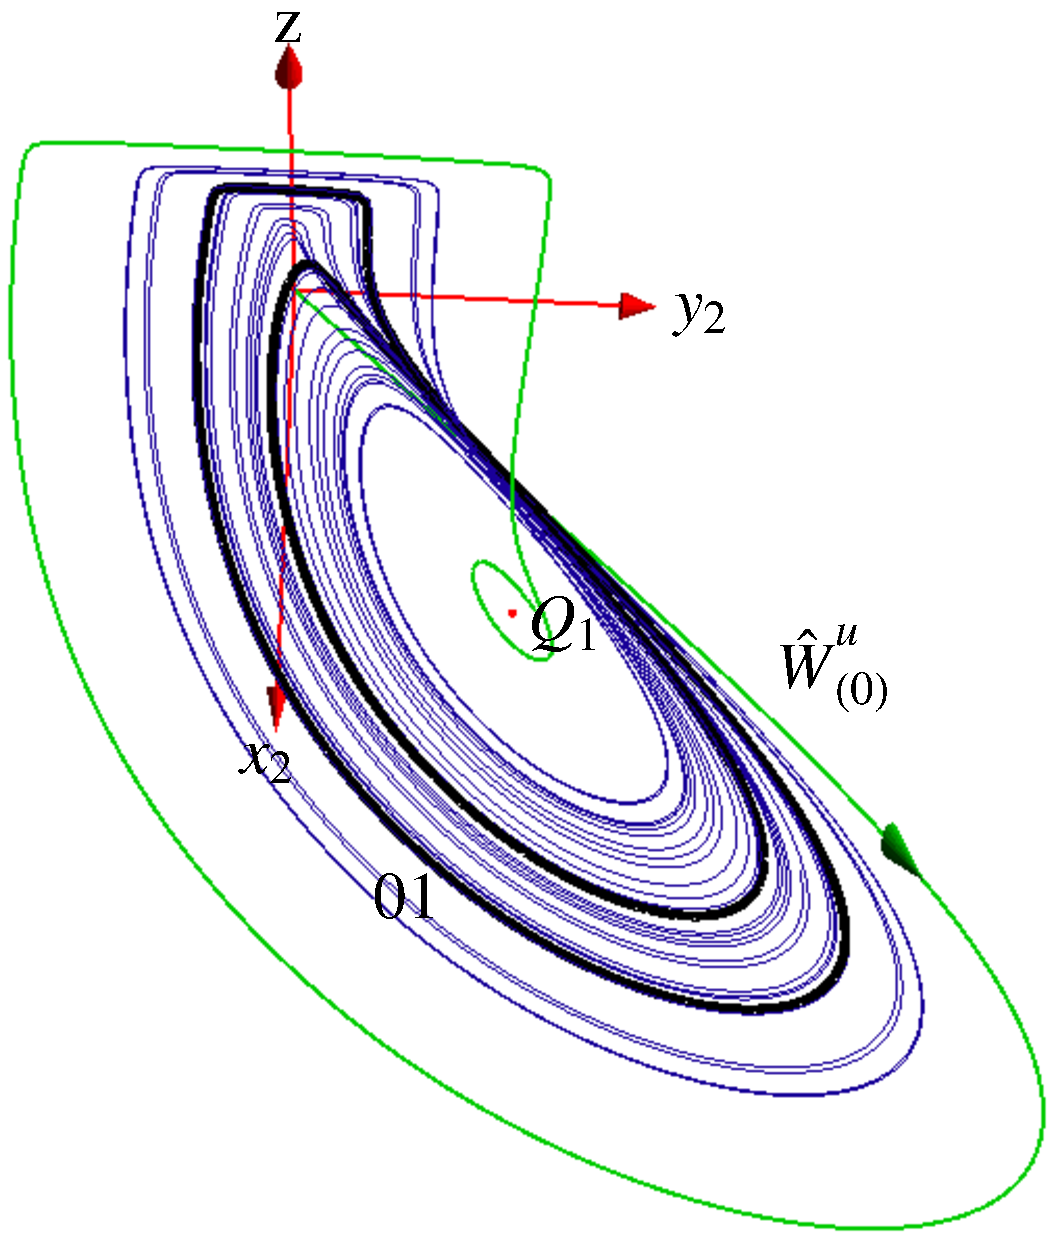
\includegraphics[width=0.6\textwidth,clip=true]
                        {CLEcoord245}
		\end{exampleblock}
	\end{columns}

\bigskip
ergodic trajectory was a mess, now the
topology is reveled
\\
\rpo\ \cycle{01} now a \po
\end{frame}

\begin{frame}{triumph : all pipe flow solution in one happy family}
\slicep\ is typical turbulent state (breaks all symmetries)
\\
plot $N2\_M1, \cdots$, \reqva, unstable manifolds
%($\Reynolds =2400$, stubby $L=2.5D$ pipe)
	\begin{columns}[t]
	\column{.50\textwidth}
\begin{block}
  \centering
\includegraphics[width=1.00\textwidth]{1611M1PROJFULL}
\\
    all in the same projection
\\
    inset: an expanded view % near the upper branch
\\
    blue loop: $T=4.93$ \\ \rpo
\end{block}
	\column{0.50\textwidth}
\begin{block}
  \centering
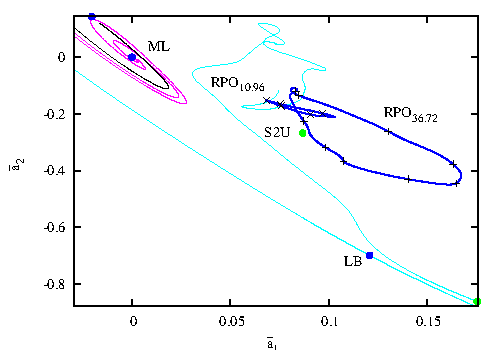
\includegraphics[width=1.00\textwidth]{2803M1projOrb}
%\label{fig:M1Orb}
\\
      $T=10.96$ and $T=36.92$
\\
\rpo s
\\
embedded in turbulence
\end{block}
	\end{columns}
\bigskip
first 'turbulent' \rpo s for pipe flows!
\end{frame}

\begin{frame}{slice trouble 1}
\begin{block}{portrait of \cLf\ in \reducedsp}
\begin{center}
(\textit{a})
  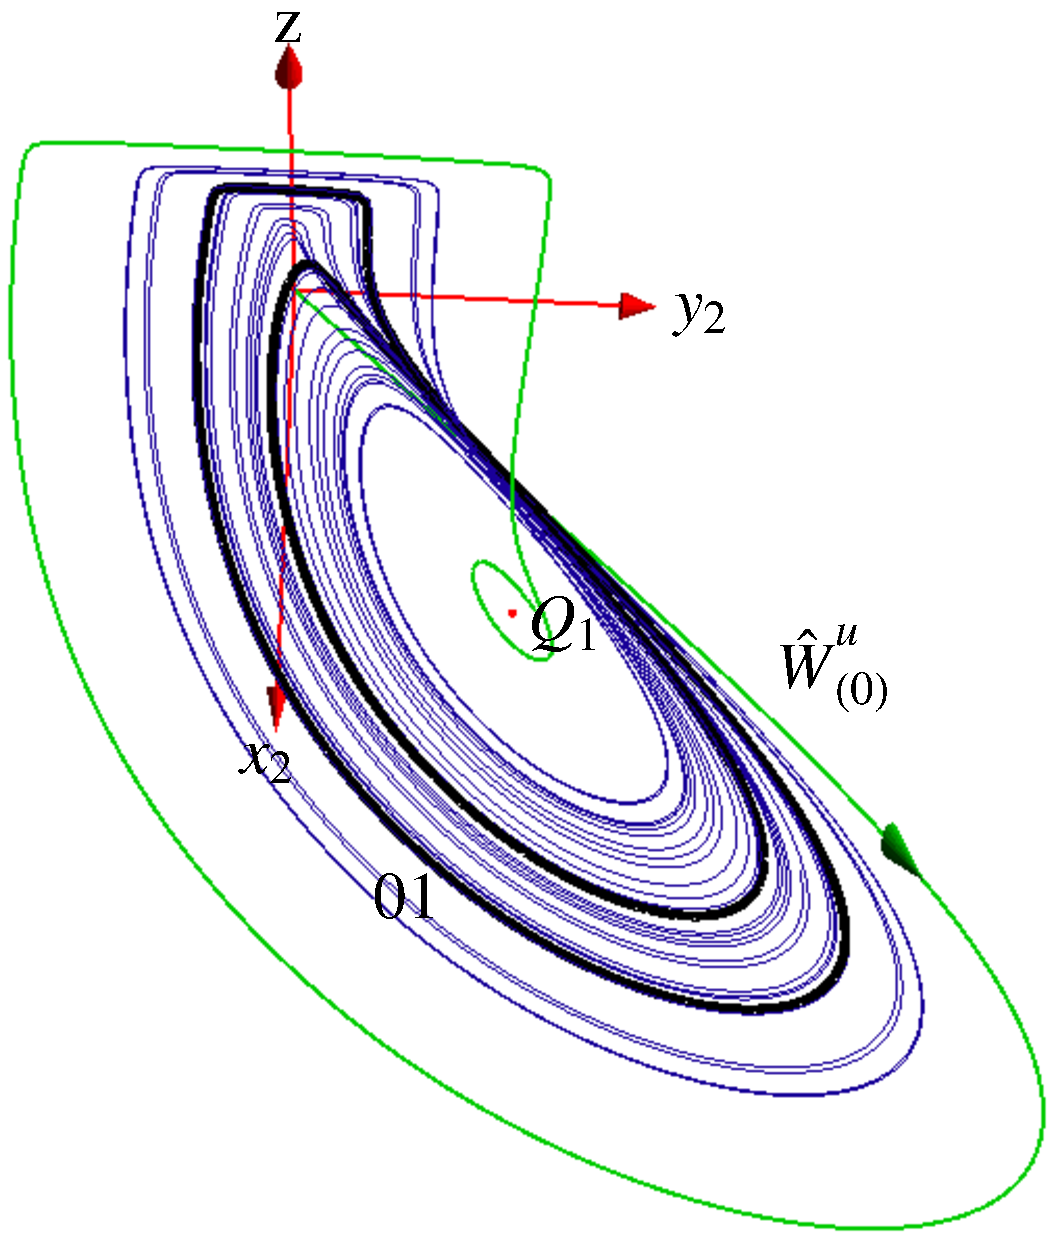
\includegraphics[width=0.40\textwidth,clip=true]
  {CLEcoord245}
(\textit{b})
  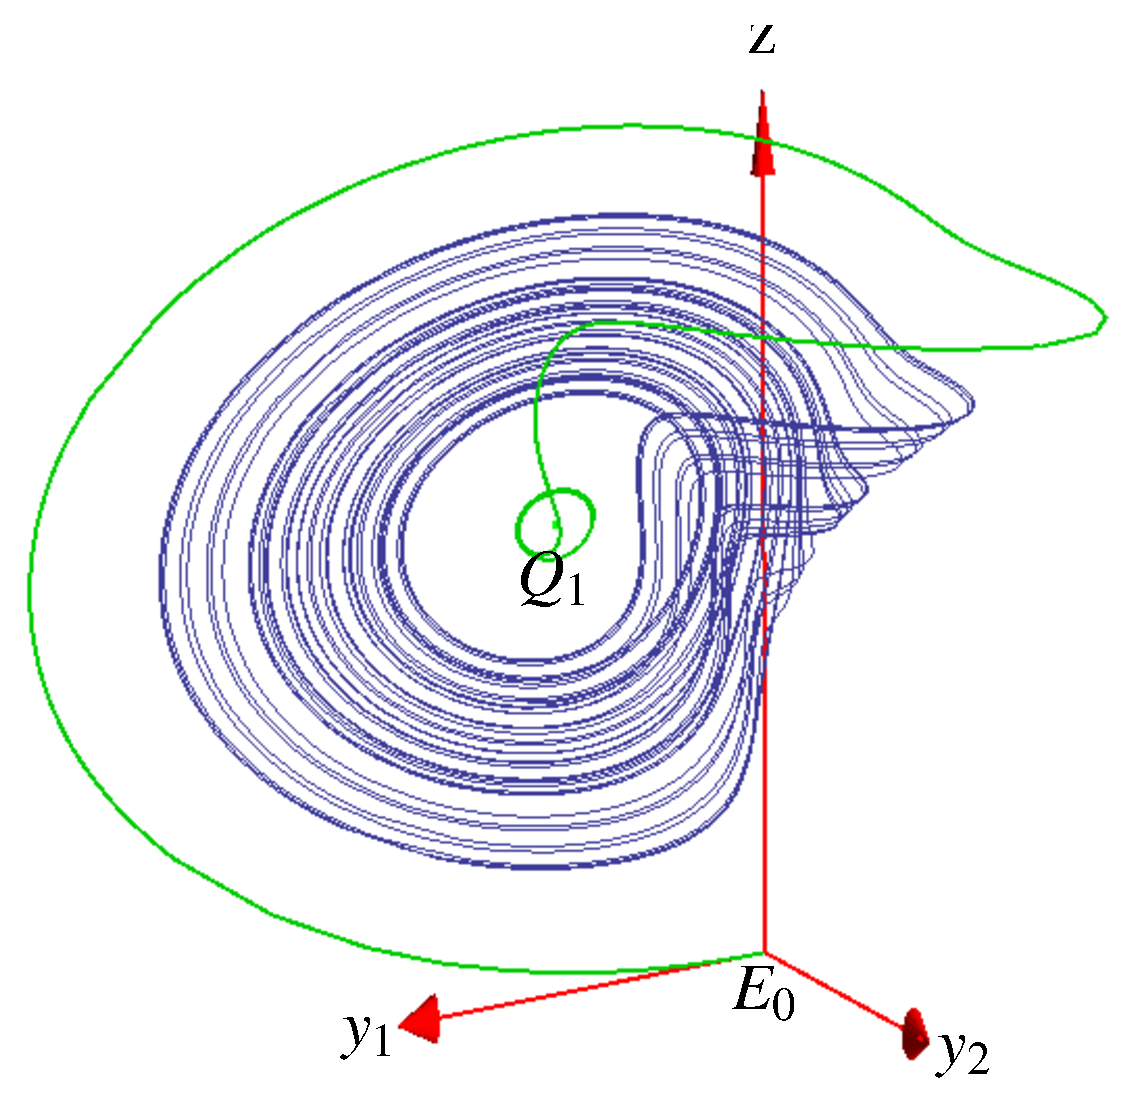
\includegraphics[width=0.45\textwidth,clip=true]
  {CLEperpReqb}
\end{center}
\end{block}
any choices of the slice $\slicep$
exhibit flow discontinuities
\end{frame}

\begin{frame}{slice trouble 1}
\begin{block}{glitches!}
group tangent of a generic trajectory orthogonal
to the slice tangent at a sequence of instants $\tau_k$
\[
\groupTan(\tau_k)^T \cdot \sliceTan{} = 0
\]
\end{block}
\end{frame}

\begin{frame}{example: group orbit of a pipe flow turbulent state}
\slicep\ is Kerswell \emph{et al} $N2\_M1$  \reqv
\\
( $\Reynolds =2400$,
stubby $L=2.5D$ pipe)
	\begin{columns}[t]
	\column{.45\textwidth}
			\begin{exampleblock}
{$\SOn{2}\times\SOn{2}$ symmetry
\\
$\Rightarrow$
group orbit is 2-torus}

\bigskip
a turbulent state
			\end{exampleblock}
\begin{block}{distance extremum condition}
$$ %beq
\frac{\partial ~~}{\partial \gSpace_a} |\ssp - \LieEl(\gSpace)\,\slicep|^2
   = 0
$$ % ee{PCsectQ0}
\end{block}
	\column{0.55\textwidth}
\begin{block}
  \centering
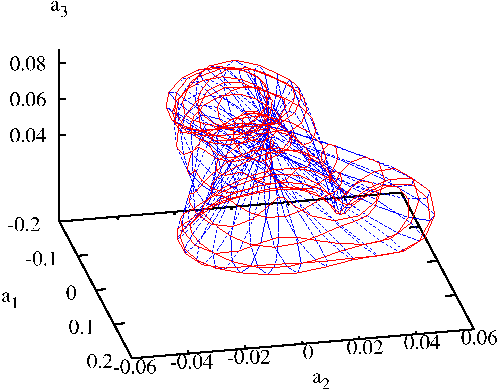
\includegraphics[width=1.20\textwidth]{2840GOt135M1} %{2830GO7}
%  \caption{\label{fig:2830GO6}
    %\label{fig:M1groupOrb}
\end{block}
	\end{columns}

\bigskip
group orbits of highly nonlinear states are highly contorted:
many extrema, multiple sections by a slice
\end{frame}

\begin{frame}{slice trouble 2}
 \begin{columns}
 \column{0.6\textwidth}
\begin{block}{slice cuts a \rpo\ multiple times}
\begin{center}
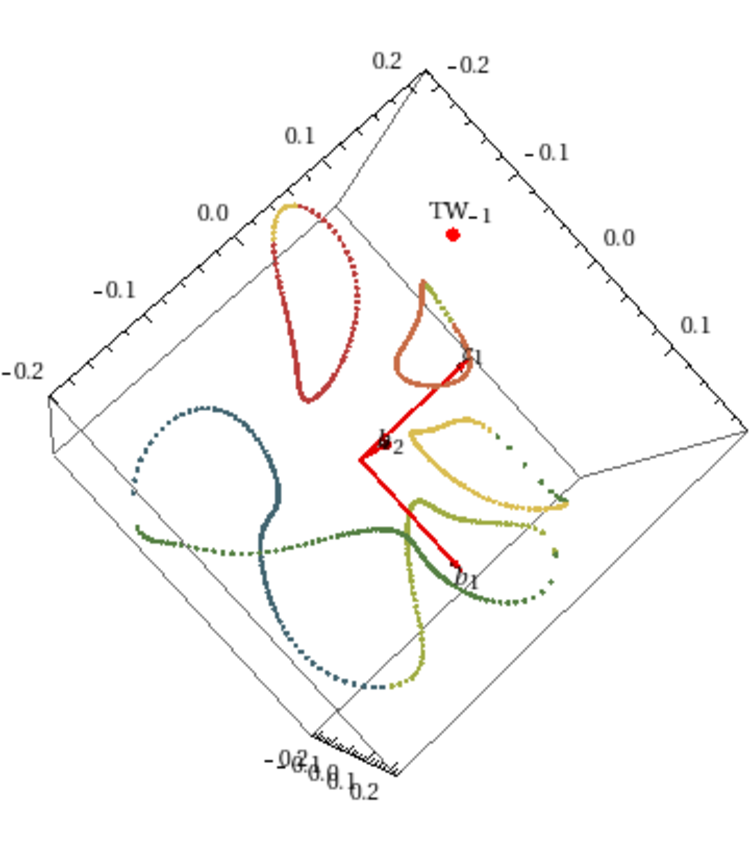
\includegraphics[width=0.80\textwidth]
            {ks22rpo16mfAll}
\end{center}
\end{block}
 \column{0.4\textwidth}
a single \rpo\ is intersected by a slice in $3$ separate sections of
the \rpo\ torus
\\
and $3$ sections that appear to connect to a closed loop
  \end{columns}
\end{frame}

\section{charting the \statesp}

\begin{frame}{trouble: slices cannot be global}
  \begin{columns}
  \column{0.70\textwidth}
\begin{block}{} %group orbits}
\begin{center}
  \includegraphics[width=1.00\textwidth,clip=true]
  {slicePhil}
\end{center}
\end{block}
  \column{0.30\textwidth}
representing a group orbit by the closest match
to a good template $\slicep$
(Phil Morrison)
\end{columns}
\end{frame}

\begin{frame}{trouble: slices cannot be global}
  \begin{columns}
  \column{0.70\textwidth}
\begin{block}{} %group orbits}
\begin{center}
  \includegraphics[width=1.00\textwidth,clip=true]
  {slicePhilY}
\end{center}
\end{block}
  \column{0.30\textwidth}
the `closest match'
to a bad template $\slicep$
(young Phil Morrison) can be a mismatch

\bigskip

\noindent
\textcolor{blue}{single template cannot be a good match  globally}
\end{columns}
\end{frame}

\begin{frame}{trouble: slices cannot be global}
  \begin{columns}
  \column{0.70\textwidth}
\begin{block}{} %group orbits}
\begin{center}
  \includegraphics[width=1.00\textwidth,clip=true]
  {slicePhil0}
\end{center}
\end{block}
  \column{0.30\textwidth}
another attempt, another bad template $\slicep$
(younger Morrison)
\end{columns}
\end{frame}

\begin{frame}{trouble: slices cannot be global}
  \begin{columns}
  \column{0.70\textwidth}
\begin{block}{} %group orbits}
\begin{center}
  \includegraphics[width=1.00\textwidth,clip=true]
  {sliceSonya}
\end{center}
\end{block}
  \column{0.30\textwidth}
representing a group orbit by the closest match
to a better template $\slicep$
(Sonya Kovalewskaya)

\bigskip

\noindent
\textcolor{blue}{to cover $\pS/\Group$ globally, need}:
\\
a set of templates:
\\\begin{itemize}
    \item 2 rolls
    \item 4 rolls
    \item ...
  \end{itemize}
\end{columns}
\end{frame}

\begin{frame}{How good is your slice?}
hyperplane of points \sspSing\ defined by being normal to  the quadratic
Casimir-weighted vector $\Lg^2\slicep$, such that from the {\template}
vantage point their group orbits are not transverse, but locally
`horizontal,'
\[ %beq
\braket{\groupTan(\sspSing)}{\sliceTan{}}
 =
-\braket{\sspSing}{\Lg^2\slicep}
 =0
%\,.
\] %ee{sliceSingl0}
{\scriptsize
(for simplicity, specialize to the  $\SOn{2}$ case)
}
\end{frame}

\begin{frame}{\sset}
%$(d\!-\!2)$\dmn\
$S$ : set of all points $\sspRSing$ which are both
\begin{itemize}
  \item[(a)] in the {\slice}
  \item[(b)] whose group tangent $\groupTan(\sspRSing)$
                is also in the  {\slice}
\end{itemize}
\bea
\braket{\sspRSing}{\sliceTan{}}&=&0 \continue
\braket{\groupTan(\sspRSing)}{\sliceTan{}}
 &=&
-\braket{\sspRSing}{\Lg^2\slicep}
 =0
% \,.
\nnu %label{sliceSingl}
\eea
$S$ is the locus of
inflection points, a hyperplane through which
\begin{itemize}
  \item curvature of the distance function changes sign
  \item local minimum turns into a local maximum
\end{itemize}
\end{frame}

\begin{frame}{\slice\ is good up to \sset}
\begin{block}{}
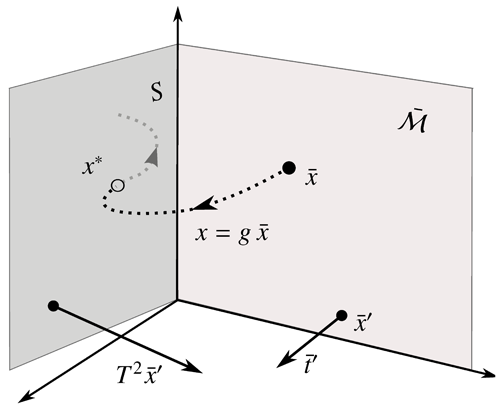
\includegraphics[width=0.80\textwidth]{inflectHype.png}
\end{block}
\end{frame}


\begin{frame}{charting the \statesp}
for turbulent/chaotic systems a set of \Poincare sections is needed to
capture the dynamics. The choice of sections should reflect the
dynamically dominant patterns seen in the solutions of nonlinear PDEs

\medskip

we propose to construct a global atlas of the dimensionally \reducedsp\
$\pSRed$ by deploying linear \Poincare sections $\PoincS{}^{(j)}$ across
neighborhoods of the qualitatively most important patterns $\slicep{}^{(j)}$
\end{frame}

\begin{frame}{}
\begin{center}
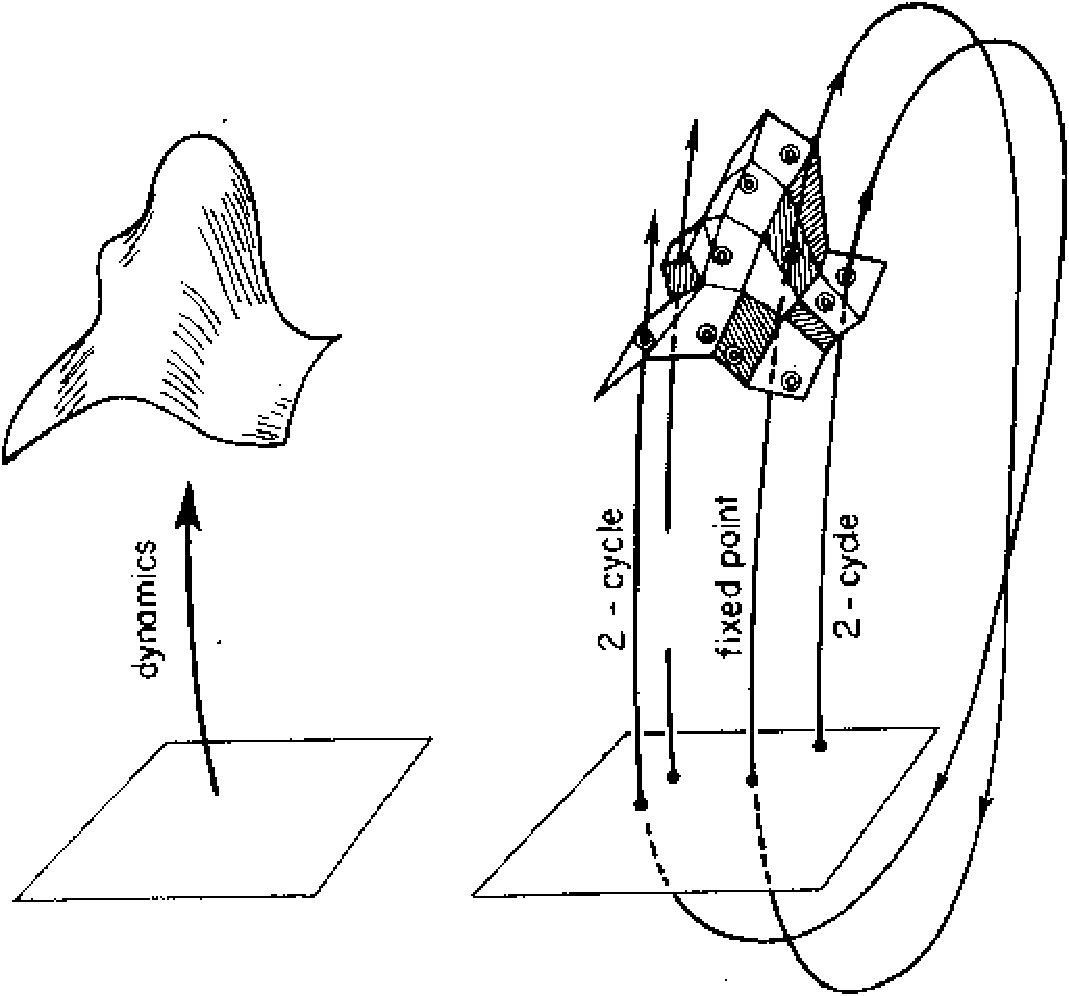
\includegraphics[width=0.60\textwidth]{f_1_08_1}
\end{center}
this is the
periodic-orbit implementation of the idea of {\statesp\ tessellation}
\end{frame}

\begin{frame}{}
we shall refer to these states as \emph{\template s}, each represented in
the \statesp\ $\pS$ of the system by a \emph{\template\ point} $\slicep$

\medskip

together with the velocity field at this point, a template defines a
linear \Poincare section, an affine hyperplane $\sspRed \in \PoincS$,
\beq
    \vel(\slicep) \cdot (\sspRed - \slicep)= 0
\,,
\ee{locTransvVar1}
locally normal to the $\vel(\slicep)$ at the \template\ point $\slicep$
\end{frame}

\begin{frame}{}
each \Poincare section $\PoincS{}^{(j)}$, provides a local chart at
$\slicep{}^{(j)}$ for a neighborhood of an important, qualitatively
distinct class of solutions (2-rolls states, 3-rolls states, \etc)

\medskip
together they `Voronoi' tessellate  the curved manifold in which the
reduced strange attractor is embedded by a finite set of hyperplane tiles
\end{frame}

\begin{frame}{}
a \Poincare section is a ($d\!-\!1$)\dmn\ hyperplane. If we pick another
{\template} point $\slicep{}^{(2)}$, it comes along with its own
\Poincare section
\medskip

any neighboring pair of $(d\!-\!1)$\dmn\ \Poincare
sections intersects in a `ridge' (`boundary,' `edge'), a $(d\!-\!2)$\dmn\
hyperplane, easy to compute
\end{frame}

\begin{frame}{}
a global atlas so constructed should be
sufficiently fine-grained: each `chart' or `tile,' bounded by ridges to
neighboring \Poincare sections, should be sufficiently small

\medskip

physical task is to, for a given dynamical flow, pick a set of
qualitatively distinct {\template s} whose \Poincare sections are locally
tangent to the strange attractor
\end{frame}

\begin{frame}{\statesp\ tessellation by \po s}
    \begin{minipage}[b]{0.40\textwidth}
\begin{block}{}
two 1-cycles

\medskip

a 2-cycle that alternates
between the neighborhoods of the two 1-cycles,
shadowing first one of the
two 1-cycles, and then the other
%}{fig:Tesselate} %{Hyp} %{fig6} and {tr:fig6} in ChaosBook
\end{block}
    \end{minipage}
~~~~~~
    \begin{minipage}[b]{0.51\textwidth}
\begin{center}
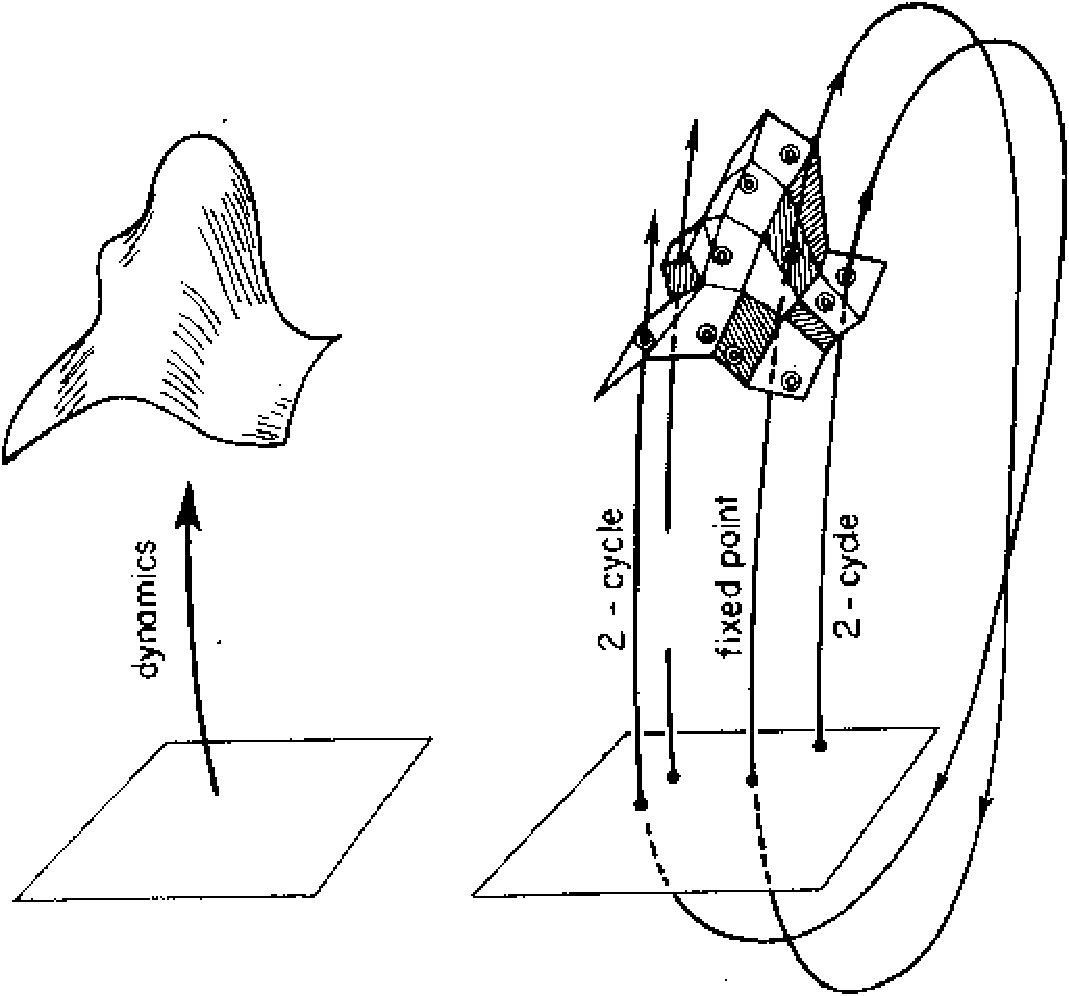
\includegraphics[width=1.00\textwidth]{f_1_08_1}
\end{center}
    \end{minipage}
smooth dynamics  (left frame) tesselated by the skeleton of periodic
points, together with their linearized neighborhoods, (right frame)
\end{frame}


\section[Summary]{conclusions}

 \begin{frame}{summary}

\begin{block}{conclusion}
  \begin{itemize}
   \item symmetry reduction by \mslices:
   \\
   efficient, allows
   exploration of high-dimensional flows\\
hitherto unthinkable
   \item stretching and folding
  	of unstable manifolds in \reducedsp\ organizes the flow
  \end{itemize}
\end{block}

\begin{block}{to be done}
\begin{itemize}
  \item construct Poincar\'e sections and return maps
  \item find all (relative) periodic orbits up to a given period
  \item use the information quantitatively (periodic orbit theory)
\end{itemize}
\end{block}
\end{frame}

\begin{frame}{take-home message}
if you have a symmetry
\begin{center}
\textcolor{red}{\Large use it!}
\end{center}

\bigskip\bigskip
without symmetry reduction, no understanding of pipe, Couette, ...,
flows possible
\end{frame}

\begin{frame}{amazing theory! amazing numerics! frustration...}
\begin{center}
  
\includegraphics[width=0.60\textwidth,clip=true]
                    {ProblemsPill}
\end{center}
\end{frame}


\section[flotsam]{flotsam - Hilbert polynomials impractical}


%\begin{frame}{unstable \rpo s}
%\Rpo s (modulated traveling waves) satisfy:
%\[
%  \Shift_{\shift_p/L}u(x,\period{p}) =
%  u(x+\shift_p,\period{p}) = u(x,0) = u_p(x)\,.
%\]
%\Po s satisfy:
%% \[
%%    \Refl u(x+\shift,\period{p}) =
%%   -u(-x-\shift,\period{p}) = u(x+\shift,0) = u_p(x)
%% \]
%\[
%   u(x,\period{p}) = u(x,0)=u_p(x)
%\]
%\end{frame}

\begin{frame}{Happy families are all alike;
             \\
             every unhappy family is unhappy in its own way}

\bigskip

everybody, her mother,
\\
and Robert MacKay knows how to do this

\bigskip

except the author of
\end{frame}

\begin{frame}{masters of group theory}
\begin{center}
  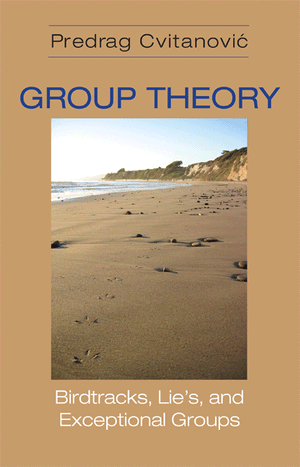
\includegraphics[width=0.40\textwidth,clip=true]
                    {coverBtracks}
\end{center}
\end{frame}

\begin{frame}{Lie groups}
all the group theory needed here is in
principle contained in
the \textcolor{blue}{Peter-Weyl theorem}:

\begin{block}{compact Lie group $\Group$}
 \begin{itemize}
   \item completely reducible
   \item its representations are fully reducible
   \item every compact Lie group is a subgroup of $U(n)$ for some
$n$
   \item every
continuous, unitary, irreducible representation of a compact Lie group is
finite dimensional
 \end{itemize}
\end{block}
\end{frame}

\begin{frame}{example: discrete symmetries of \pCf}
%{     \label{exmp:pCfSymmDiscr}
Navier-Stokes equations for
the \pCf\  have two discrete symmetries,
in addition to the two continuous translational symmetries:
rotation by $\pi$ in the (streamwise,spanwise) plane, and
rotation by $\pi$ in the (streamwise,wall-normal) plane

\bigskip
that is why there exist \eqva\ (as opposed to
\reqva) and some periodic orbits in the \pCf

\bigskip
they belong to discrete symmetry subspaces

\bigskip
a \rpo\ can be pre-periodic if it is invariant under a discrete symmetry:
If ${g}^m=1$ is of finite order
$m$, then the corresponding orbit is periodic with period $m\period{p}$.
\end{frame}

\begin{frame}{example: symmetries of \pCf}
%{    \label{exmp:PpCfSymm}
 		\begin{exampleblock}{}
Navier-Stokes flow between two countermoving planes

\bigskip
        \includegraphics[width=.80\textwidth,clip=true]
                        {PCF-geometry-presentation} %CLEx1x2zRelEqu}
		\end{exampleblock}

\bigskip
\begin{itemize}
  \item box periodic in
streamwise and spanwise directions
  \item eqs. invariant under streamwise, spanwise flips
  \item $\On{2}\times \On{2}$ continuous symmetry
\end{itemize}
\end{frame}

\begin{frame}{example: group orbits of \pCf}
%{    \label{exmp:PpCfSymm}
	\begin{columns}[t]
	\column{.6\textwidth}
			\begin{exampleblock}{\pCf}
flow periodic in streamwise and spanwise directions
			\end{exampleblock}
	\column{.40\textwidth}
 		\begin{exampleblock}{}
        \includegraphics[width=\textwidth,clip=true]
                        {PCF-geometry-presentation} %CLEx1x2zRelEqu}
		\end{exampleblock}
	\end{columns}
\begin{itemize}
  \item $\SOn{2}\times \SOn{2}$ continuous symmetry
  \item each \eqv/\reqv\ $\in$ 2-torus of equivalent solutions
  \item a relative periodic solution recurs at
time $\period{p}$ with exactly the same disposition of velocity fields
over the entire box, but shifted by a 2-dimensional (streamwise,spanwise)
translation $g_p$
\end{itemize}
\end{frame}

\begin{frame}{}
group action ${g_p}$ is referred to as a ``phase,'' or a ``shift''

\bigskip
continuous symmetry
parameters $\{t,\gSpace_1,\cdots,\gSpace_N\}$ are
real numbers, ratios $\pi/\gSpace_j$ are almost never rational, and
\rpo s are almost never eventually periodic
\end{frame}

\begin{frame}{}
$\sspRed$ is the point on the group orbit of $\ssp$
\[ %beq
\ssp=\LieEl(\gSpace)\,\sspRed
	\,,\qquad
\LieEl \in \Group
\,,
\] %\ee{sspOrbit}
closest to the {\template} {\slicep}, the Lie group element
$\LieEl=\LieEl(\gSpace)\propto\exp{({\gSpace} \cdot \Lg)}$
\end{frame}

\begin{frame}{symmetry reduction methods}
the key result of the representation theory
of invariant functions

\begin{block}{Hilbert-Weyl theorem}
For a compact group $\Group$ there exist a finite
$\Group${-invariant} homogenous polynomial basis
$\{u_1,u_2, \dots,u_m\}$ such that any $\Group${-invariant} polynomial
can be written as a multinomial
\beq
h(\ssp) = p(u_1(\ssp),u_2(\ssp), \dots,u_m(\ssp))
\,.
\ee{HilbWeyl}
\end{block}

\medskip

explicit construction of such basis is often not feasible,
and we will not take this path except for a few simple
low-dimensional cases
\end{frame}

\begin{frame}{}
we propose to construct a global atlas by deploying a set of
linear \Poincare sections and slices in neighborhoods of the most important
equilibria and/or periodic orbits as local charts
\end{frame}

\begin{frame}{reduction methods}
\begin{enumerate}
	\item  {\bf Hilbert polynomial basis}: rewrite equi\-vari\-ant
dynamics in in\-vari\-ant coordinates\only<2>{:
\textcolor{green}{global, but useless in dimension larger than 10}
        }
	\item {\bf moving frames, or slices}:
cut group orbits by a hypersurface (kind of
Poincar\'e section), each group orbit of
symmetry-equivalent points represented by the single point\only<2>{:
\textcolor{red}{local}
        }
\end{enumerate}
\end{frame}

\begin{frame}{slice \& dice}
\begin{block}{flow reduced to a slice}
\begin{center}
  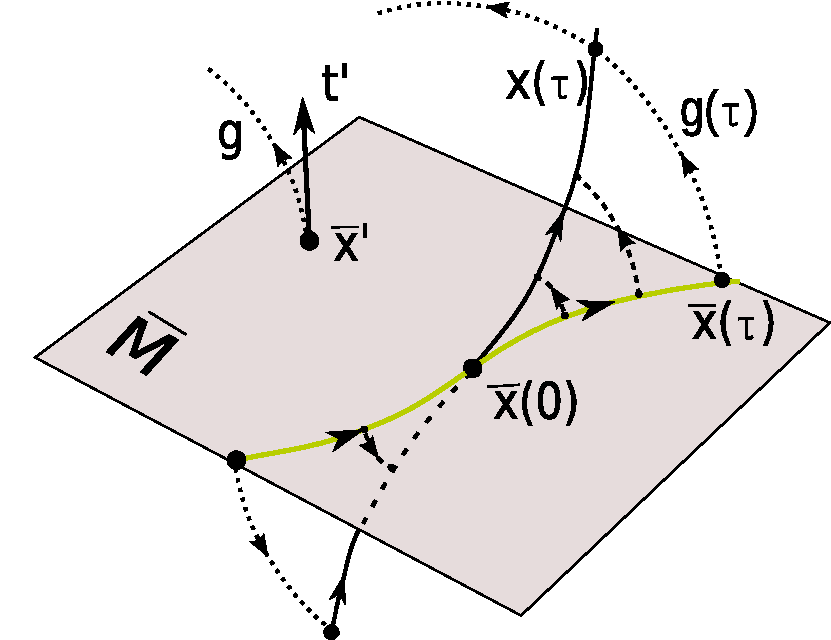
\includegraphics[width=0.45\textwidth,clip=true]
  {ReducTraj3}
\end{center}
\end{block}
\slice\ \pSRed\
through the slice-fixing point $\slicep$,
normal to the group tangent $\sliceTan{}$ at $\slicep$,
intersects
group orbits (dotted lines).
The full
\statesp\ trajectory $\ssp(\tau)$ and the \reducedsp\
trajectory $\sspRed(\tau)$ are equivalent up to a group rotation
$\LieEl(\tau)$.
\end{frame}

% \begin{frame}{Moving frame method}
%  \begin{block}{Idea}
%   	\begin{itemize}
%  		\item Introduce a \emph{cross-section}: A hypersurface that intersects all group
% 			orbits of a point exactly once.
% 		\item Then given a point $x$ find a map that tells you the transformation parameter(s)
% 			needed to bring $x$ to the cross-section. This is called a moving frame.
% 	\end{itemize}
%  \end{block}
%
%  \begin{block}{For \CLe}
% 	\begin{description}
%  		\item{Cross-section} $x_1=0$, $x_2>0$.
% 		\item{Moving frame} $\theta=\tan^{-1}\frac{x_1}{x_2}$.
% 	\end{description}
%   	
%  \end{block}


% \end{frame}

% \begin{frame}{Moving frame method}
%
% % \[
% % 	\left(\barr{cc} \overline{b}_k \\ \overline{c}_k\earr \right)=\left(\barr{cc}
% % 			    			\cos(k\theta) & -\sin(k\theta)\\
% % 						\sin(k\theta) & \cos(k\theta)\\
% % 			   			\earr\\	
% % 						\right) \left(\barr{cc} b_k \\ c_k\earr\right)\,,\ \ k=1,\ldots N\,.
% % \]
% % with $a_k=b_k+i c_k\,,\ b_k,c_k\in\Rls{}$.
% \end{frame}

\end{document}
